\documentclass[conference]{IEEEtran}
\IEEEoverridecommandlockouts
% Document Class: IEEEtran 2015/08/26 V1.8b by Michael Shell
% -- http://www.michaelshell.org/tex/ieeetran/

\usepackage{cite}
\usepackage{amsmath,amssymb,amsfonts}
\usepackage{algorithmic}
\usepackage{graphicx}
\usepackage{textcomp}
\usepackage{xcolor}
\usepackage{float}
\usepackage{filecontents}
\usepackage{kotex}
\usepackage{lipsum}

\documentclass{scrreprt}
\makeatletter
\usepackage{color}
\definecolor{lightgray}{rgb}{0.95, 0.95, 0.95}
\definecolor{darkgray}{rgb}{0.4, 0.4, 0.4}
%\definecolor{purple}{rgb}{0.65, 0.12, 0.82}
\definecolor{editorGray}{rgb}{0.95, 0.95, 0.95}
\definecolor{editorOcher}{rgb}{1, 0.5, 0} % #FF7F00 -> rgb(239, 169, 0)
\definecolor{editorGreen}{rgb}{0, 0.5, 0} % #007C00 -> rgb(0, 124, 0)
\definecolor{orange}{rgb}{1,0.45,0.13}		
\definecolor{olive}{rgb}{0.17,0.59,0.20}
\definecolor{brown}{rgb}{0.69,0.31,0.31}
\definecolor{purple}{rgb}{0.38,0.18,0.81}
\definecolor{lightblue}{rgb}{0.1,0.57,0.7}
\definecolor{lightred}{rgb}{1,0.4,0.5}
\usepackage{upquote}
\usepackage{listings}
% CSS
\lstdefinelanguage{CSS}{
  keywords={color,background-image:,margin,padding,font,weight,display,position,top,left,right,bottom,list,style,border,size,white,space,min,width, transition:, transform:, transition-property, transition-duration, transition-timing-function},	
  sensitive=true,
  morecomment=[l]{//},
  morecomment=[s]{/*}{*/},
  morestring=[b]',
  morestring=[b]",
  alsoletter={:},
  alsodigit={-}
}

% JavaScript
\lstdefinelanguage{JavaScript}{
  morekeywords={typeof, new, true, false, catch, function, return, null, catch, switch, var, if, in, while, do, else, case, break},
  morecomment=[s]{/*}{*/},
  morecomment=[l]//,
  morestring=[b]",
  morestring=[b]'
}

\lstdefinelanguage{HTML5}{
  language=html,
  sensitive=true,	
  alsoletter={<>=-},	
  morecomment=[s]{<!-}{-->},
  tag=[s],
  otherkeywords={
  % General
  >,
  % Standard tags
	<!DOCTYPE,
  </html, <html, <head, <title, </title, <style, </style, <link, </head, <meta, />,
	% body
	</body, <body,
	% Divs
	</div, <div, </div>, 
	% Paragraphs
	</p, <p, </p>,
	% scripts
	</script, <script,
  % More tags...
  <canvas, /canvas>, <svg, <rect, <animateTransform, </rect>, </svg>, <video, <source, <iframe, </iframe>, </video>, <image, </image>, <header, </header, <article, </article
  },
  ndkeywords={
  % General
  =,
  % HTML attributes
  charset=, src=, id=, width=, height=, style=, type=, rel=, href=,
  % SVG attributes
  fill=, attributeName=, begin=, dur=, from=, to=, poster=, controls=, x=, y=, repeatCount=, xlink:href=,
  % properties
  margin:, padding:, background-image:, border:, top:, left:, position:, width:, height:, margin-top:, margin-bottom:, font-size:, line-height:,
	% CSS3 properties
  transform:, -moz-transform:, -webkit-transform:,
  animation:, -webkit-animation:,
  transition:,  transition-duration:, transition-property:, transition-timing-function:,
  }
}

\lstdefinestyle{htmlcssjs} {%
  % General design
%  backgroundcolor=\color{editorGray},
  basicstyle={\footnotesize\ttfamily},   
  frame=b,
  % line-numbers
  xleftmargin={0.75cm},
  numbers=left,
  stepnumber=1,
  firstnumber=1,
  numberfirstline=true,	
  % Code design
  identifierstyle=\color{black},
  keywordstyle=\color{blue}\bfseries,
  ndkeywordstyle=\color{editorGreen}\bfseries,
  stringstyle=\color{editorOcher}\ttfamily,
  commentstyle=\color{brown}\ttfamily,
  % Code
  language=HTML5,
  alsolanguage=JavaScript,
  alsodigit={.:;},	
  tabsize=2,
  showtabs=false,
  showspaces=false,
  showstringspaces=false,
  extendedchars=true,
  breaklines=true,
  % German umlauts
  literate=%
  {Ö}{{\"O}}1
  {Ä}{{\"A}}1
  {Ü}{{\"U}}1
  {ß}{{\ss}}1
  {ü}{{\"u}}1
  {ä}{{\"a}}1
  {ö}{{\"o}}1
}
%
\lstdefinestyle{py} {%
language=python,
literate=%
*{0}{{{\color{lightred}0}}}1
{1}{{{\color{lightred}1}}}1
{2}{{{\color{lightred}2}}}1
{3}{{{\color{lightred}3}}}1
{4}{{{\color{lightred}4}}}1
{5}{{{\color{lightred}5}}}1
{6}{{{\color{lightred}6}}}1
{7}{{{\color{lightred}7}}}1
{8}{{{\color{lightred}8}}}1
{9}{{{\color{lightred}9}}}1,
basicstyle=\footnotesize\ttfamily, % Standardschrift
numbers=left,               % Ort der Zeilennummern
%numberstyle=\tiny,          % Stil der Zeilennummern
%stepnumber=2,               % Abstand zwischen den Zeilennummern
numbersep=5pt,              % Abstand der Nummern zum Text
tabsize=4,                  % Groesse von Tabs
extendedchars=true,         %
breaklines=true,            % Zeilen werden Umgebrochen
keywordstyle=\color{blue}\bfseries,
frame=b,
commentstyle=\color{brown}\itshape,
stringstyle=\color{editorOcher}\ttfamily, % Farbe der String
showspaces=false,           % Leerzeichen anzeigen ?
showtabs=false,             % Tabs anzeigen ?
xleftmargin=17pt,
framexleftmargin=17pt,
framexrightmargin=5pt,
framexbottommargin=4pt,
%backgroundcolor=\color{lightgray},
showstringspaces=false,      % Leerzeichen in Strings anzeigen ?
}%
%
\makeatother

\begin{document}

\title{MulMeokNyang\\
{\footnotesize \textsuperscript{}Intelligent cat watering machine that Recognizes individual cats with AI}
}

\author{\IEEEauthorblockN{Ann Jukyung}
\IEEEauthorblockA{\textit{Dept. Information Systems} \\
\textit{Hanyang University}\\
Seoul, South Korea \\
email@hanyang.ac.kr}
\and
\IEEEauthorblockN{Choi Chansol}
\IEEEauthorblockA{\textit{Dept. Information Systems} \\
\textit{Hanyang University}\\
Seoul, South Korea \\
email@hanyang.ac.kr}
\and
\IEEEauthorblockN{Lee Yunsun}
\IEEEauthorblockA{\textit{Dept. Information Systems} \\
\textit{Hanyang University}\\
Seoul, South Korea \\
email@hanyang.ac.kr}
\and
\IEEEauthorblockN{Hong JunGgi}
\IEEEauthorblockA{\textit{Dept. Information Systems} \\
\textit{Hanyang University}\\
Seoul, South Korea \\
sentorino@hanyang.ac.kr}
}

\maketitle

\begin{abstract}
Cats are known for their discerning palates and can be quite selective, particularly when it comes to wet food, especially if they haven't been exposed to a variety of flavors previously. This dietary preference, coupled with a reluctance to consume adequate water, can lead to dehydration and pose a significant threat to feline health. To address this issue, smart cat water dispensing systems aim to offer a solution through the identification and in-depth analysis of individual cats' unique preferences and hydration needs.
\end{abstract}

\begin{IEEEkeywords}
identification, detection, classification, opencv, cats
\end{IEEEkeywords}

\section{Role Assignment}
Roles are assigned to improve software development process and increase team productivity. Group name is called Nyangporter.
\newline

% add description if needed
\begin{table}[!htbp]\normalsize
\begin{center}
\begin{tabular}{|p{1.2cm}|p{1.9cm}|p{4.5cm}|}
\hline
\textbf{Name} & \textbf{\textit{Role}}& \textbf{\textit{Responsibilities}}\\
\hline
Choi Chansol & Development manager &
The role involves task allocation, project progression assessment, translating requirements into practical functionality, and discerning the most suitable frameworks for the project.\newline 
\newline This position also encompasses the execution of software features and active collaboration with co-workning Software Developers to deliver essential functionalities.
\\ \hline
\end{tabular}
\label{tab1}
\end{center}
\end{table}
\newpage
\begin{table}[!htbp]\normalsize
\begin{center}
\begin{tabular}{|p{1.2cm}|p{1.9cm}|p{4.5cm}|}
\hline
Ann Jukyung & Software developer &
This role primarily involves implementing software features and collaborating with fellow developers to meet feature requirements. Additionally, it includes the vital task of ensuring that the minimum viable product remains on schedule. \newline
\newline This position is also responsible for engaging with users and customers to gather and integrate feedback into the product's development process. Code maintenance and overseeing the coordination of pull requests are also integral aspects of this role.
\\ \hline
Lee Yunsun & User &
Tasked with app testing and identifying any deficiencies that require enhancement, this role also involves offering goals, expectations, and deliverables for improving these weaknesses and ensuring ongoing compliance with requirements. \newline 
\newline Should the requirements fall short of expectations, the individual is responsible for communicating actionable feedback and evaluating implemented features.
\\ \hline
\end{tabular}
\label{tab2}
\end{center}
\end{table}
\newpage
\begin{table}[htbp!]\normalsize
\begin{center}
\begin{tabular}{|p{1.2cm}|p{1.9cm}|p{4.5cm}|}
\hline
Hong JunGgi & Customer &
This role is responsible for thoroughly testing the application, not only for functionality but also for usability, design, and overall user experience. This testing process allows for a comprehensive assessment, providing valuable insights that can guide improvements and refinements in various aspects of the application, ensuring it meets the user's distinct needs and requirements more effectively.
\\ \hline
\end{tabular}
\label{tab3}
\end{center}
\end{table}

\section{INTRODUCTION}
\subsection{Motivation}


Cats tend to consume only the least amount of water, and due to this lack of drinking water, they often have health problems and have to go to the hospital regularly. Since animals are not applied by insurance, the burden of owners is considerable. In addition, in order to increase the amount of water consumed, the owners make them drink wet feed or force them to drink water through injections, but some cats suffer from allergic reactions to wet feed, and they show severe rejection to forced water intake by injection. \\
So we need a natural way to increase the amount of water consumed. Also, the number of households raising companion animals is increasing these days due to the increase in single or two-person households. \\

Therefore, we will proceed this project so that households with cats can manage the amount of water consumed by cat through smart cat water supply machine and mobile applications. \\

\subsection{Problem Statement}
Though there are some exceptions, most cats are particularly susceptible to becoming dehydrated as they abhor drinking water like other animals do. Smart cat water supply machine is a project aiming to recognize individual cats and analyze their water consumption data in order to make sure they are consuming appropriate amounts of food and water to avoid dehydration. We envision Smart cat water supply machines to allow clients, especially with more than two or more cats, to have access to cats' water consumption data easily and notify them if they may be in a threatening condition. \\

In the existing pet water supply system, only one animal per water supply system could be managed because there was no individual identification function in case of raising multiple cats and dogs in one household. With this in mind, our team will recognize the faces of multiple pets to enable differentiated negative number management for each individual. \\

Our goal is to provide clients with an application that can monitor their cats’ water consumption data individually and hopefully give clients information on cats’ health conditions. Identification will be done by embedding a camera on the feeder product and capturing cats’ faces to analyze their facial features through Machine Learning. This solution will be able to help both clients and cats themselves by being able to monitor their water intake easily and providing them with necessary information regarding cats' health condition. \\

\subsection{Research on any related software}

The AI cat feeding product landscape is indeed populated with various existing solutions, reflecting the strong interest of pet owners in this field. However, it's important to note that the majority of these solutions fall into two categories: not AI, commercially-driven products, and non-open source projects. It was either too simple to be called Artificial Intelligence or AI part was very confidential.
\newline

\subsubsection*{VaraemPet's Welli Smart Hydration Care}

In response to the central proposition concerning the daily water intake recommendation for humans, this innovative AI-driven pet hydration monitoring system seeks to address the vital question of how to ensure our pets' proper hydration. This system offers comprehensive hydration monitoring, enabling pet owners to precisely gauge their pets' hydration levels in comparison to recommended averages. It meticulously records and evaluates crucial data, including food intake, water consumption, and weight, all consolidated within a comprehensive health record. Furthermore, it provides real-time notifications via the Baraem app, keeping pet owners updated each time their pets drink and offering valuable insights into their hydration patterns. To facilitate a deeper understanding of their pet's hydration trends, the app displays detailed daily, weekly, and monthly hydration graphs, along with comparisons against peer averages. Additional features encompass monitoring remaining water levels and issuing timely cleaning notifications. The system's adjustable height feature caters to pets of various sizes, ensuring a comfortable drinking experience. Moreover, it follows a standard hydration formula based on the pet's weight, recommending a daily water intake of (Weight x 50 ml). It's important to note that the product's limitation lies in its inability to provide individual identification for multi-pet households, which means it cannot differentiate or tailor services for each pet separately.
\newline

\newpage

\section{REQUIREMENTS ANALYSIS}
\subsection{Sign up}
\begin{itemize}
\item{\emph{Basic Information Input Screen:}}
    \begin{itemize}
        \item Method 1) Quick Sign-Up Feature
        \begin{itemize}
            \item Utilizes the Kakao, Google, and Naver sign-up APIs.
            \item If a quick sign-up is done, it directly proceeds to the user profile setup screen.
        \end{itemize}
        \item Method 2) Local Sign-Up Feature
        \begin{itemize}
            \item Email Input: The system checks and displays whether the input is in the correct email format or if the email has already been registered.
            \item Password and Password Confirmation Input: The system checks if both values match and displays the result on the screen.
            % \item Phone Number Input and Authentication: Uses the NICE mobile phone authentication API. Once the authentication is complete, it displays the result on the screen.
        \end{itemize}
        \item If all the fields are correctly filled out and authentication is complete, the "Next" button is activated, leading the user to the user profile setup screen. \newline 
    \end{itemize}
\item{\emph{User Profile Setup Screen:}}
    \begin{itemize}
        \item Profile Picture Registration (optional)
            \begin{itemize}
            \item Clicking the "Add Photo" button allows the user to either fetch a photo from the album or take one instantly with the camera. The chosen photo can then be registered.
            \item If no photo is registered separately, a default image is displayed. - Nickname Input (Required)
            \end{itemize}
        \item Nickname Input (Required)
            \begin{itemize}
            \item The system checks the format and checks for duplicates, then displays the result on the screen.
            \end{itemize}
        \item Self-Introduction Input (optional)
            \begin{itemize}
            \item A maximum character count is specified.
            \end{itemize}
        \item If the nickname is correctly entered, the "Complete Sign-Up" button is activated. After sign-up, the user starts from the <water dispenser device registration> screen in a logged-in state and proceeds through the cat hydration management space creation procedure.\\
    \end{itemize}
\end{itemize}

\subsection{Login}
\begin{itemize}
\item{\emph{Method 1) Quick Login:}}
\item{\emph{Method 2) Local Login}}
    \begin{itemize}
        \item The system checks whether the email address and password have been entered.
        \item If entered, the system verifies if there's a matching user in the database.
        \item If no match is found, the user is prompted to re-enter. If a match is found, a cookie is generated to maintain the logged-in state continuously.
        \item If the auto-login checkbox is checked, a session is generated to remember the login details, and upon logging out, the login details are automatically filled in.
        \item After successful login, if the user has their own space or is a part of any, they are directed to the cat hydration management space.
        \item Otherwise, they begin from the water dispenser device registration screen and proceed through the cat hydration management space creation procedure.\\
    \end{itemize}
\end{itemize}

\subsection{Find Email}
\begin{itemize}
% \item First, authenticate the user using the NICE Mobile Phone Verification API.
\item Upon successful authentication, the system searches the database using the phone number and displays the user's email on the screen.\\
\end{itemize}

\subsection{Forgot Password}
\begin{itemize}
\item Enter the email address for which you want to retrieve the password.
\item After authentication, the system searches the database using the email and phone number, and then sends the user's password to the specified email.\\
\end{itemize} 

\subsection{Water Dispenser Device Registration}
(Step 1 of Creating a Cat Hydration Management Space)
\begin{itemize}
\item Instruct the user to put the water dispenser device into pairing mode.
    \begin{itemize}
        \item Provide a picture indicating the location of the pairing button on the dispenser.
    \end{itemize}
\item Search for available water dispenser devices and display them in a list.
\item The user selects the desired device from the list.
\item Once paired successfully, register the device information in the application and then navigate to the cat profile registration screen.\\
\end{itemize}

\subsection{Cat Profile Registration}
(Step 2 of Creating a Cat Hydration Management Space)
\begin{itemize}
\item{\emph{Basic Information Entry Screen}}
    \begin{itemize}
        \item Register a profile picture of the pet cat, and enter its name, weight, and age.
        \item Once all details are entered, the next button is activated, allowing the user to proceed to the Nose Print Photo Registration screen.
    \end{itemize}
\item{\emph{Nose Print Photo Registration Screen}}
    \begin{itemize}
        \item Uses Nose Print Recognition AI model.
        \item To identify the individual cat, submit multiple photos of the cat's nose from various angles.
        \item After uploading the photos, you can press the next button to proceed to the Wet Food Intake Information Registration screen.
    \end{itemize}
\item{\emph{Wet Food Intake Information Entry Screen}}
    \begin{itemize}
        \item Select 'Yes/No' for consumption status.
        \item If 'No' is selected, activate the "Next" button.
        \item If 'Yes' is selected, input the daily intake amount in grams and the moisture content of the food. Once all details are entered, activate the "Next" button.
        \begin{itemize}
            \item If the moisture content is unknown, a default value of 70\% is set.
        \end{itemize}
        \item Clicking the "Next" button leads to the hydration setting screen.
    \end{itemize}
\item{\emph{Hydration Setting Screen}}
    \begin{itemize}
        \item Choose between 'Automatic setting/Manual setting'.
        \item If 'Automatic setting' is chosen, the recommended hydration formula is applied, and the "Next" button gets activated.
        \begin{itemize}
            \item Daily basis formula: `( Weight(kg) * 50ml ) - ( Wet food amount (g) * Moisture content(\%) )`
        \end{itemize}
        \item If 'Manual setting' is chosen, users input the daily target hydration amount, and then the "Next" button gets activated.
        \item Add another cat button:
        \begin{itemize}
            \item Redirects to the second cat profile registration screen.
        \end{itemize}
        \item Complete profile registration button:
        \begin{itemize}
            \item Directs to the cat hydration management space.\\
        \end{itemize}
    \end{itemize}
\end{itemize}

\subsection{Cat Hydration Management Space (Main)}
\subsubsection{Daily Hydration Info for Each Cat}
\begin{itemize}
    \item Cat Profile Selection Top Bar
    \begin{itemize}
        \item By tapping the profile picture, users can access the hydration info screen for that specific cat.
    \end{itemize}
    \item Cat Profile
    \begin{itemize}
        \item Displays the cat's profile picture, name, age, and weight.
        \item An edit button lets users access a screen where they can modify that cat's profile. (Reuses the Cat Profile Registration screen).
        \item Tapping the right arrow displays the daily hydration info for the next cat. The last item is a plus button, which leads to a screen to add a new cat profile. (Reuses the Cat Profile Registration screen).
    \end{itemize}
    \item Daily Hydration Gauge
    \begin{itemize}
        \item Displays how much of the daily hydration goal the cat has achieved, as a percentage(\%).
        \item Different colors indicate hydration ranges:
        \begin{itemize}
            \item 0\% ~ 29\%: Red
            \item 30\% ~ 59\%: Yellow2
            \item 60\% ~ 89\%: Green
            \item 90\% ~ Upper Limit: Blue
            \item Upper Limit ~ 200\%: Blue up to the upper limit, then red
        \end{itemize}
        \item The upper limit is set to address excessive hydration, calculated using the recommended formula.
        \item Push notifications are sent to the user if the upper limit is exceeded.
    \end{itemize}
    \item Daily Hydration Evaluation \& Advice
    \begin{itemize}
        \item Based on the cat's water intake for the day, an evaluation is given, advising if more water intake is needed.
    \end{itemize}
    \item Hydration Statistics Button
    \begin{itemize}
        \item Leads to the periodical hydration statistics screen for that cat.
    \end{itemize}
    \item Watering Attempt Button
    \begin{itemize}
        \item Tapping this button prompts the water dispenser to make a cat-calling sound, enticing the cat to approach and drink.
        \item If the cat drinks within 30 minutes, a push notification is sent to the user.
    \end{itemize}
    \item Navigation Bar
    \begin{itemize}
        \item Tapping the NavigationBarIcon slides out the navigation bar from the left.\\
    \end{itemize}
\end{itemize}
\subsubsection{Periodical Hydration Statistics Screen}
\begin{itemize}
    \item Cat Profile Selection Top Bar
    \begin{itemize}
        \item If accessed from a specific cat's daily hydration info screen, that cat is selected.
        \item Otherwise, the first cat is selected by default.
        \item Users can view statistics for other cats by selecting their profiles.
    \end{itemize}
    \item By default, displays a bar graph of the past week's hydration data.
    \item Users can choose between 'One Week/One Month/One Year' durations.
    \item A calendar button allows users to select specific 'Week/Month/Year'.
    \item Tapping a bar displays hydration data for that specific 'Day/Week/Month'.
    \begin{itemize}
        \item If the graph is set for one week, it displays data for that day.
        \item If set for one month, it displays data for that week.
        \item If set for one year, it displays data for that month.
    \end{itemize}
    \item At the bottom, an evaluation and advice on hydration are provided.
    \begin{itemize}
        \item If 'Red' or 'Yellow' days make up more than half, a message suggests increasing water intake.
        \item If 'Green' or 'Blue' days make up more than half, a message confirms adequate hydration.
        \item If days with 'Blue + Red' make up more than half, a message advises consulting with a veterinarian due to excessive water intake.\\
    \end{itemize}
\end{itemize}

\subsection{Navigation}
To quickly transition to the desired screen, navigation links are provided in the navigation bar. The navigation bar is applied to screens where necessary, providing relevant links for each screen.\newline
\begin{itemize}
\item User Profile: Displays the user's nickname, email, profile picture, and self-introduction.
\item Menu Link List:
    \begin{itemize}
        \item Profile Management: Takes the user to a screen where they can modify their profile.
        \begin{itemize}
            \item (Reuses the User Profile Setup screen from the sign-up process)
        \end{itemize}
        \item Cat Profile Management: Takes the user to a screen where they can modify the cat's profile.
        \begin{itemize}
            \item (Reuses the Cat Profile Registration screen)
        \end{itemize}
        \item Today's Hydration Info: Takes the user to the screen that displays the day's hydration information.
        \item Hydration Statistics: Takes the user to the screen that displays periodic hydration statistics.
        \item Co-admin Management: Takes the user to the Co-admin Management screen.
    \end{itemize}
    \item Logout Button:
    \begin{itemize}
        \item Upon selection, the app processes the logout and redirects the user to the initial screen (Sign-up and Login).\\
    \end{itemize}
\end{itemize}

\subsection{Co-admin Management}
To enable the use of the Cat Hydration Management Space at the family level, a co-admin feature is provided.\newline
\begin{itemize}
\item Co-admin Profile Card List
    \begin{itemize}
        \item Each card displays the co-admin's profile picture, nickname, and self-introduction.
        \item There is a delete button on the card, which, when pressed, removes the co-admin rights for that user.
    \end{itemize}
\item Add Co-admin Button
    \begin{itemize}
        \item Pressing this button brings up a dialog box prompting the user to enter the nickname of the co-admin they wish to add.
        \item If the entered nickname exists in the system, that user will be added as a co-admin. If the nickname does not exist, the user will be prompted to re-enter a valid nickname.
        \item Once a co-admin is added, a push notification is sent to that user.
        \item When the newly added co-admin logs into the app, if auto-login is set, they are immediately directed to the Cat Hydration Management Space to which they belong.\\
    \end{itemize}
\end{itemize}

\newpage
\section{Development Environment}
% add description if needed
\subsection{Choice of software development platform}
We are using windows 11 environment, we are likely to use bash terminal or WSL most of the time. Other tools like vscode or jupyter notebook will be based on windows 11. Windows might not be the best choice for software development environment but it is considered one of the good option and we don't have linux machine so we had no choice. In addition, Visual Studio Code will be used as IDE, and Typescript, Python, and MySQL will be used as languages.

\begin{table}[!htbp]\normalsize
\begin{center}
\begin{tabular}{|p{1.4cm}|p{6.2cm}|}
\hline
\textbf{Tool and language} & \textbf{\textit{Reason}}\\
\hline
Typescript & Typescript is an open-source programming language that is a super-set of JavaScript. By specifying the static type, type errors can be prevented, high code readability, and errors can be checked during compilation. It is also a class-based object-oriented programming language that can support inheritance, encapsulation, and generator. Since all the team members are familiar with JavaScript, and Typescript is a complementary language to JavaScript, we chose to learn it through this opportunity 
\\ \hline
React Native & React Native can develop platform applications and is partially compatible native. It was judged that developing Android and IOS applications in native languages was less efficient, and the accessibility of developing React Native was high due to the knowledge of React. In addition, it is a framework that is widely used in the field, so we chose it as the front-end language.
\\ \hline
Expo & Expo is a React Native cross platform for development. It was judged that Xcode was not available because we do not have a Mac OS device, and it was inefficient because it was not suitable for the project size to develop using both Android studio and Xcode. With Expo, IOS applications can be developed in Windows as well, and real-time tests can be made with mobile devices held through the Expo application. In addition, it was used because the initial setting was simple and there were many modules needed to develop the Expo SDK.
\\ \hline
\end{tabular}
\label{tab1}
\end{center}
\end{table}
\newpage

\begin{table}[!htbp]\normalsize
\begin{center}
\begin{tabular}{|p{1.8cm}|p{5.8cm}|}
\hline
Node.js & Node.js is commonly used by back-end development beginners because it can quickly process data with an asynchronous event-based architecture and provides most of what is needed in package manager. Most of the team members does not have back-end development experience and have knowledge of JavaScript, so we decide to use Node.js. Using Nest.js that supports Typescript as a framework, we hope to facilitate co-working with front-end developers who use React Native.
\\ \hline
MySQL & We need a database to store the user information, user's cat information, list of co-manager, and water consumption data. MySQL is an open-source relational database system language, we decide to use because all team members have used it in the "Database System" class.
\\ \hline
Amazon Web Services(AWS) & To back up and manage databases by building and hosting cloud-based servers, we intend to use Amazon Relational Database Service (RDS) and Amazon SageMaker to manage machine learning services. With SageMaker, data scientists and developers can quickly and easily build and train machine learning models, and then directly deploy them into a production-ready hosted environment. We can get a 12-month Free Tier also a reason for choice.
\\ \hline
Python 3.11 & Python is an interpreted, object-oriented, high-level programming language with dynamic semantics. Because Python is simple to use and it can be used in Machine Learning development, its popularity in AI and ML development is very high. We will be using libraries like matplotlib for visualization, tensorflow/pytorch for image classification, scikit-learn for data analysis, and all the rest of the necessary libraries like pandas or numpy etc.
\\ \hline
\end{tabular}
\label{tab1}
\end{center}
\end{table}
\textit{Cost Estimation}
\newline
We will use open source if possible, and servers will also use AWS Free Tier plans to avoid incurring development costs.
\newline
\subsection{Software in use}
\begin{itemize}
\item[a.]{\emph{Visual Studio Code(1.83.1)}}
   \newline
   Visual Studio Code (VSCode) is an open-source IDE and can be used in various environments such as Windows, macOS, and Linux. In addition to code editing, it supports various development tasks such as debugging, version management, and terminal access, also there are many extension plug-ins that can increase development productivity with plug-ins such as Prettiers. We chose this IDE because the OS of laptops used by team members is different, also it would be easy for everyone to use the same IDE for smooth cooperative working.
    \\ \end{itemize}
\begin{itemize}
\item[b.]{\emph{SKT NUGU}}
   \newline
   SKT NUGU is an artificial intelligence(AI) service based on voice recognition. It was intended to increase the user's convenience by notifying the amount of water consumption of cats through the voice of the water supplier even without accessing the application. SKT NUGU has the advantage of providing guidelines for developers to utilize, allowing them to mount artificial intelligence-based functions easily and quickly, and being able to test without NUGU devices in a GUI environment called Play Builder.
   \\ \end{itemize}
\begin{itemize}
\item[c.]{\emph{Git hub}}
   \newline
   A version management system based on Git that allows multiple developers to work simultaneously, track changes, and avoid conflicts. The remote storage provided enables collaboration online, and facilitates communication between team members, code review, and issue management. We hope to use GitHub to prevent version problems during collaboration and to check and develop each other's code.
    \\ \end{itemize}
\begin{itemize}
\item[d.]{\emph{Database Management System}}
   \newline
   A database management system is essential to manage the information of the user, the user's cats, and cats’ water consumption data. To easily and securely store the information associated with it, the database needs to be designed and built.
    \\ \end{itemize}
\begin{itemize}
\item[e.]{\emph{Figma}}
   \newline
   Figma is a web-based UI/UX design tool. It supports many designers and developers to collaborate in real-time, and does not require installation. It is easy to build and manage reusable components, making it possible to maintain a consistent design pattern, which also contributes to increasing developer productivity. In addition, it is available for free and is not difficult to use, so we chose it as a software design tool.
    \\ \end{itemize}
\begin{itemize}
\item[f.]{\emph{Open CV}}
   \newline
   This is a library of programming functions mainly for real-time computer vision. We found other alternatives like YOLOv8. However, it is unclear whether it could be used or not due to my limitation on knowledge and time. For now, we are looking to use built-in Haar Cascade alorithm for object detection.
    \\ \end{itemize}
    
\newpage
\subsection{Task distribution}
\begin{table}[!htbp]\normalsize
\begin{center}
\begin{tabular}{|p{1.2cm}|p{1.9cm}|p{4.5cm}|}
\hline
\textbf{Name} & \textbf{\textit{Role}}& \textbf{\textit{Responsibilities}}\\
\hline
Choi Chansol & Front-end &
The role involves developing mobile apps for Android and iOS using React Native. It includes UI/UX design, feature integration, and communication with the backend server via RESTful API for seamless functionality.
\\ \hline
Ann Jukyung \& Lee Yunsun & Back-end &
The responsibilities for this role encompass various aspects of software development and database management. This includes database design and management, which involves overseeing and organizing user information, device information, and statistical data. Additionally, this position involves server-client communication. This multifaceted role entails not only creating and managing the database structure but also maintaining efficient server-client communication for a seamless and responsive user experience.
\\ \hline
Hong Jun Ggi & AI &
The development environment for this project comprises Python 3.11 within a WSL (Windows Subsystem for Linux) setup. The core objective involves individual cat recognition based on unique nose prints. To achieve this, various libraries are employed, including OpenCV 4 for image processing and the likely integration of scikit-learn (sklearn) for machine learning capabilities. Additionally, for data visualization and analysis, visualization libraries like Matplotlib are utilized. Furthermore, the project explores the realm of generative AI (OpenAI API), possibly in collaboration with SKT NUGU, to enhance its capabilities and further its objectives.
\\ \hline
\end{tabular}
\label{tab2}
\end{center}
\end{table}

\section{SPECIFICATIONS}
\subsection{Database Structure}
The list below is the tables and schemes for MulMeokNyang database. When creating tables that need to be created in advance and cat's drink measurement management spaces, there are tables that need to be created dynamically.   \\

Tables that need to be generated in advance include a user table to store data for membership users and a session table to store data related to the automatic login function. \\

Tables that need to be dynamically generated include a management\_space table to store basic data related to management space, a cat\_in\_management\_space table to store basic data for cats to manage in management space, and a cat\_hydration\_statistics table to store data related to the drinking volume of a specific cat. Tables that need to be created dynamically are created together sequentially, and the table name includes the values of the spaceId and catId variables. This allows you to dynamically create and associate tables by management space and individual cat. \\

\subsubsection{Lists of tables that must be created in advance}
\begin{itemize}
    \item user table
    \begin{itemize}
        \item user\_email : primary key, not null, unique
        \item user\_pw : not null
        \item user\_name : not null
        \item user\_phonenum : not null, unique
        \item user\_profile\_photo
        \item user\_nickname : not null, unique
        \item user\_introduction
        \item management\_space\_id : default ‘’(Empty String)
    \end{itemize}
    \item session table
    \begin{itemize}
        \item session\_id : primary key, not null, unique
        \item user\_email : foreign key, not null, unique\\
    \end{itemize}
\end{itemize}
\subsubsection{Lists of tables that are going to be created statically}
\begin{itemize}
    \item management\_space\_\$\{spaceId\} table
    \begin{itemize}
        \item management\_space\_id : primary key, default \$\{spaceId\}
        \item main\_manager\_user\_email : foreign key, not null
        \item co\_managers\_user\_email : JSON, default ‘\{\}’
    \end{itemize}
    \item cat\_in\_management\_space\_\$\{spaceId\} table
    \begin{itemize}
        \item session\_id : primary key, not null, unique
        \item cat\_id : primary key, auto\_increment, default 0
        \item cat\_profile\_photo : not null
        \item cat\_name : not null
        \item cat\_age : not null
        \item cat\_weight : not null
        \item cat\_photos : JSON, default ‘\{\}’
        \item cat\_feedstuff\_daily\_consumption : not null
        \item cat\_feedstuff\_moisture\_content : not null88
        \item is\_hydration\_auto : not null
        \item cat\_goal\_hydration : not null
    \end{itemize}
    \item cat\_hydration\_statistics\_\$\{catId\} table
    \begin{itemize}
        \item date : primary key, CURDATE()
        \item day : default DAYOFWEEK(NOW())
        \item goal\_hydration : not null
        \item actual\_hydration : default 0
        \item hydration\_guage : default 0
    \end{itemize}
\end{itemize}

\subsection{Navigation}
In our application, it uses the Navigation module from the react-navigation package. \\

\subsubsection{Main Navigation}
\begin{itemize}
    \item Route List
    \begin{itemize}
        \item Start
        \item Login
        \item LocalSignUp
        \item UserProfileRegistration
        \item Find
        \begin{itemize}
            \item FindEmail
            \item FindEmailResult
            \item FindPw
        \end{itemize}
        \item HowToGoSpace
        \item PendingCoManagerAddition
        \item DeviceRegistration
        \item CatInfoRegistration
        \begin{itemize}
            \item CatProfileRegistration
            \item CatPhotosRegistration
            \item CatFeedStuffRegistration
            \item CatHydrationRegistration
        \end{itemize}
        \item Main
        \item HydrationStatistics \\
    \end{itemize}
\end{itemize}

\subsubsection{Drawer Navigation}
\begin{itemize}
    \item Route List
    \begin{itemize}
        \item UserProfileModification
        \item CatInfoRegistration
        \begin{itemize}
            \item CatProfileRegistration
            \item CatPhotosRegistration
            \item CatFeedStuffRegistration
            \item CatHydrationRegistration
        \end{itemize}
        \item CatInfoModification
        \begin{itemize}
            \item CatProfileModification
            \item CatFeedStuffModification
            \item CatHydrationModification
        \end{itemize}
        \item CoManagerSet \\
    \end{itemize}
\end{itemize}

\subsection{Frequently Used Custom Component}
The following five Component are Custom Component used throughout our application. \\

\subsubsection{TopBar Component}
\begin{itemize}
    \item[] 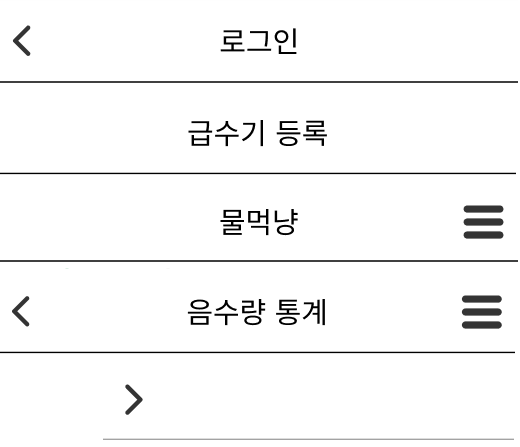
\includegraphics[width=0.3\textwidth]{img/C/1.png}
    \item The title of the current screen appears in the center, and depending on what the current screen is, go back icon and menu icon are visible.
    \item It's also used in Drawer Navigation, where it turns into a close icon rather than a backward one. \\
\end{itemize}

\subsubsection{InputContainer Component}
\begin{itemize}
    \item[] 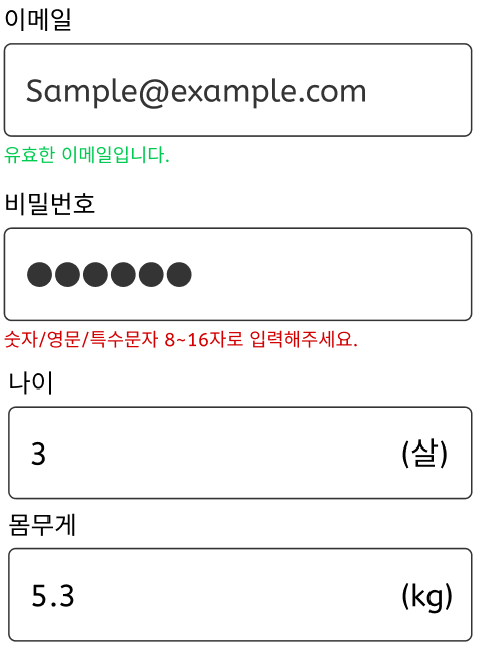
\includegraphics[width=0.27\textwidth]{img/C/2.png}
    \item Used on the Login, Sign Up, and Information Registration page.
    \item The title on the top of the page represents what that input page is for and if input requirement is not satisfied, msg will deliver information on how to satisfy those input requirements.
    \item Input values such as password and password verification are made invisible.
    \item If the input window requires a unit, the unit is shown on the right.
    \item On each screen, it passes the required validation function to properly proceed with the validation. If the validation fails, the form submit button is not activated. \\
\end{itemize}

\subsubsection{Button Component}
\begin{itemize}
    \item[] 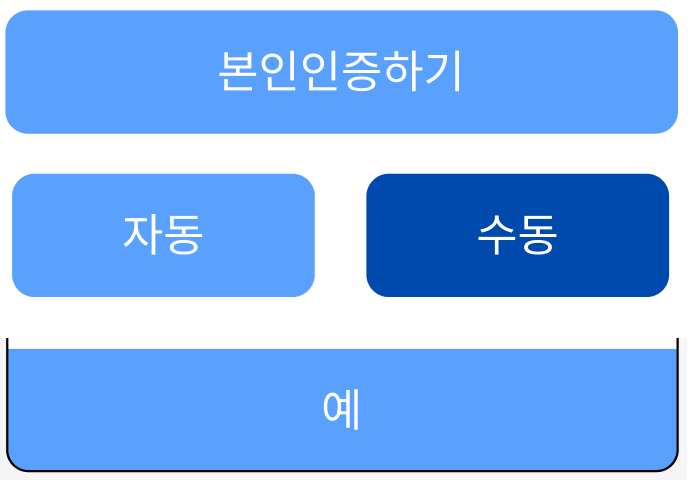
\includegraphics[width=0.25\textwidth]{img/C/3.png}
    \item Title appear and indicate which button this is inside the button.
    \item Pressing the button changes the color to navy.
    \item When it is triggered by Alert Component, it replaces the border raidus to 0.
    \item The button type includes a button to move to the specific page and a button to select a value. This is distinguished by passing the goRoute for screen movement in method property and the selectOpt value for value selection.\\
\end{itemize}

\subsubsection{Alert Component}
\begin{itemize}
    \item[] 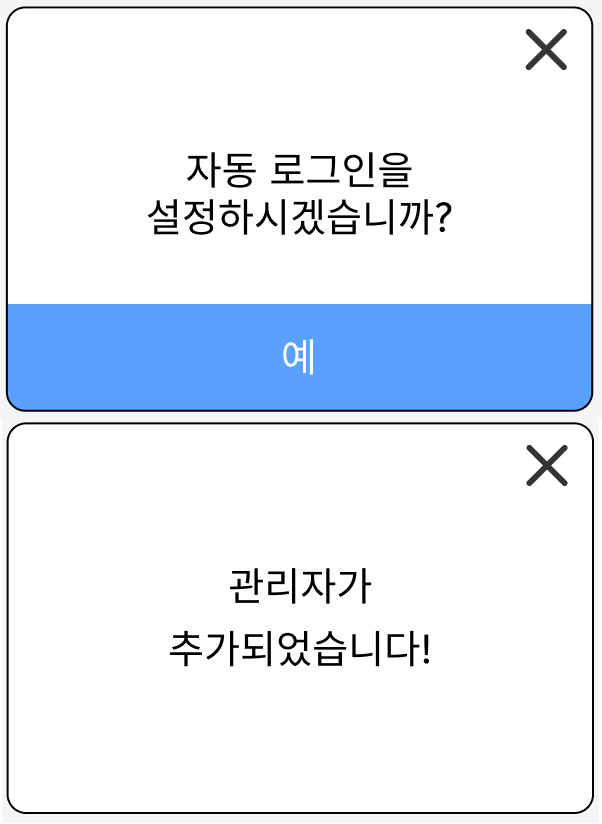
\includegraphics[width=0.2\textwidth]{img/C/4.png}
    \item Before setting up auto login or submitting a form, it appears in the form with the button.
    \item Once the data is registered or modified in the database after submitting the form, the database notifies you that the processing is complete.
    \item If you need to move to the specific page, when you press the button or close the icon, it passes the route name of the destination page to the goRoute property. \\
\end{itemize}

\subsubsection{CatProfileList Component}
\begin{itemize}
    \item[] 
\includegraphics[width=0.3\textwidth]{img/C/5.png}
    \item When you select a cat to display drink amount information on the Main Screen and Hydration Statistics Screen or when you select a cat to modify or delete information, CatProfileList appears.
    \item When the number of cats increases that the page overflows, scroll feature is available.
    \item When a cat is selected, the catId value of that cat is stored in the global variable currentSelectedCat. \\
\end{itemize}
\newpage

\subsection{Components and Configuration of each pages and Flow}
The API that requires a detailed description of the API's call and processing process is described in detail in Section E.

\subsubsection{Start Screen}
\begin{itemize}
    \item[] 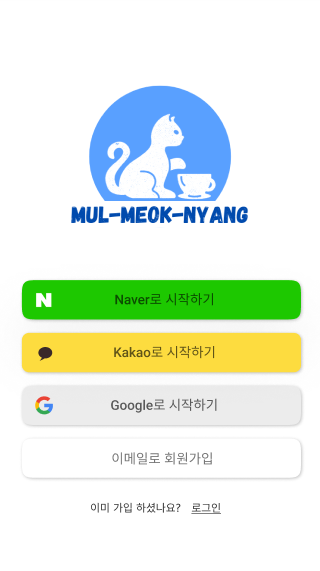
\includegraphics[width=0.27\textwidth]{img/D/1.png}
    \item Components Structure of Screen
    \begin{itemize}
        \item Image Component
        \item SignUpButton Component
        \begin{itemize}
            \item Quick SignUp and Local SignUp is distinguished with method property.
        \end{itemize}
        \item Text Component
        \item UnderlineTextButton Component
    \end{itemize}
    \item Flow of Screen
    \begin{itemize}
        \item When the app starts, it makes sure that there is a cookie in the React Native App storage.
        \item If cookie exists, it calls the AutoLogin API because user has auto-login enabled.
        \item When the button ‘\_\_\_\_\_로 시작하기’ is pressed, QuickSignUp API is called.
        \item When the button ‘이메일로 회원가입’ is pressed, it moves to the LocalSignUp Screen.
        \item When the button ‘\underline{로그인}’ is pressed, it moves to the Login Screen. 
        \\
    \end{itemize}
\end{itemize}
\newpage

\subsubsection{Login Screen}
\begin{itemize}
    \item[] 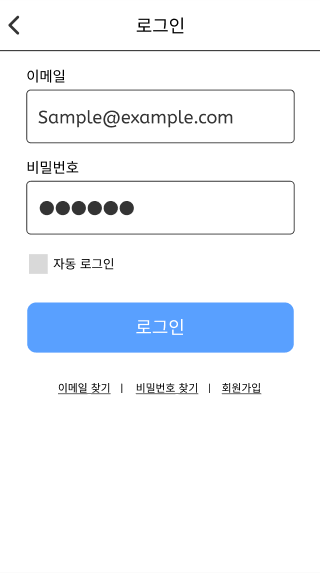
\includegraphics[width=0.27\textwidth]{img/D/2.png}
    \item Components Structure of Screen
    \begin{itemize}
        \item TopBar Component
        \item InputContainer Component
        \begin{itemize}
            \item On the Login screen, only checkEmpty validation is performed, and the results of the check is not displayed below the input box.
        \end{itemize}
        \item AutoLoginCheckbox Component
        \item Button Component
        \item UnderlineTextButton Component
    \end{itemize}
    \item Flow of Screen
    \begin{itemize}
        \item Press the Go Back button to return to the previous Screen.
        \item Enter your email and password, select whether to log-in automatically, and press the 'Log in' button to call the Login API.
        \item When the button ‘\underline{이메일 찾기}’ is pressed, moves to the FindEmail Screen.
        \item When the button ‘\underline{비밀번호 찾기}’ is pressed, moves to the FindPw Screen.
        \item When the button ‘\underline{회원가입}’ is pressed, moves to the LocalSignUp Screen.
        \\
    \end{itemize}
\end{itemize}
\newpage

\subsubsection{LocalSignUp Screen}
\begin{itemize}
    \item[] 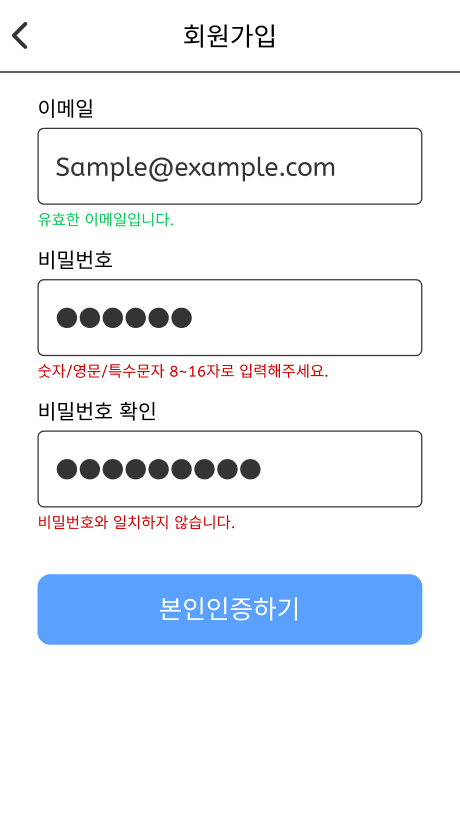
\includegraphics[width=0.27\textwidth]{img/D/3.png}
    \item Components Structure of Screen
    \begin{itemize}
        \item TopBar Component
        \item InputContainer Component
        \begin{itemize}
            \item On the LocalSignUp Screen, checkEmail, checkPw, checkConrefmPw validation is performed, and the results are displayed below the input box.
        \end{itemize}
        \item Button Component
    \end{itemize}
    \item Flow of Screen
    \begin{itemize}
        \item Press the Go Back button to return to the previous Screen.
        \item After entering e-mail, password, and password verification, press the '본인인증하기' button to call the LocalSignUp API.
        \\
    \end{itemize}
\end{itemize}
\newpage

\subsubsection{UserProfileRegistration Screen}
\begin{itemize}
    \item[] 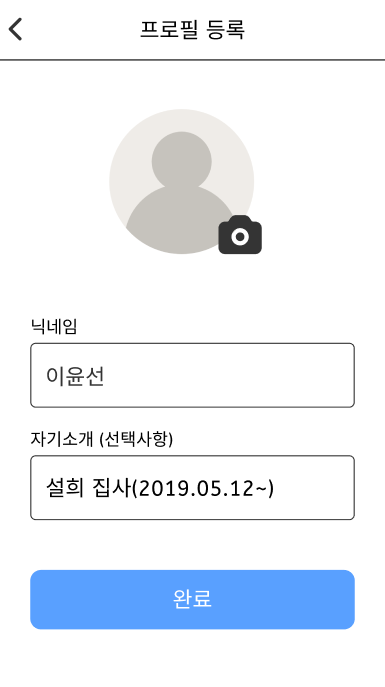
\includegraphics[width=0.27\textwidth]{img/D/4.png}
    \item Components Structure of Screen
    \begin{itemize}
        \item TopBar Component
        \item PhotoRegist Component
        \begin{itemize}
            \item Uses react-native-image-picker package.
        \end{itemize}
        \item InputContainer Component
        \begin{itemize}
            \item On the UserProfileRegistration Screen, only the nickname performs a checkEmpty validation, and the result of the check is not displayed below the input box.
        \end{itemize}
        \item Button Component
    \end{itemize}
    \item Flow of Screen
    \begin{itemize}
        \item Press the Go Back button to return to the previous Screen.
        \item Press the camera button to select a picture from the gallery, or to register a profile picture by taking a picture with the camera.
        \item Enter the nickname, which is mandatory, and press the '완료' button to call the RegisterUserProfile API.
        \\
    \end{itemize}
\end{itemize}
\newpage

\subsubsection{FindEmail Screen}
\begin{itemize}
    \item[] 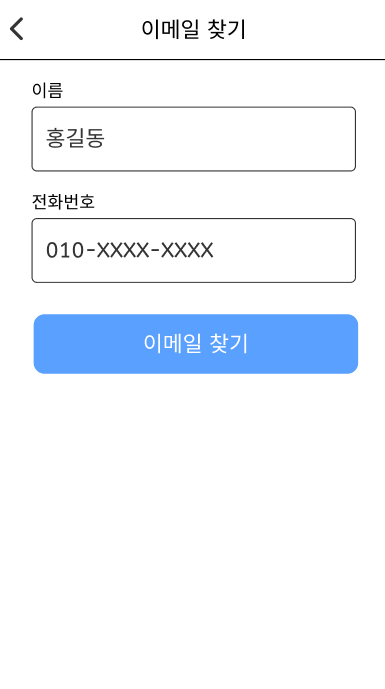
\includegraphics[width=0.27\textwidth]{img/D/5.png}
    \item Components Structure of Screen
    \begin{itemize}
        \item TopBar Component
        \item InputContainer Component
        \begin{itemize}
            \item On the FindEmail screen, checkEmpty, checkPhoneNum validation is performed, and the results of the inspection are not displayed below the input box.
        \end{itemize}
        \item Button Component
    \end{itemize}
    \item Flow of Screen
    \begin{itemize}
        \item Press the Go Back button to return to the previous Screen.
        \item Enter your name and phone number, and press the '이메일 찾기' button to call the FindEmail API.
        \\
    \end{itemize}
\end{itemize}
\newpage

\subsubsection{FindEmailResult Screen}
\begin{itemize}
    \item[] 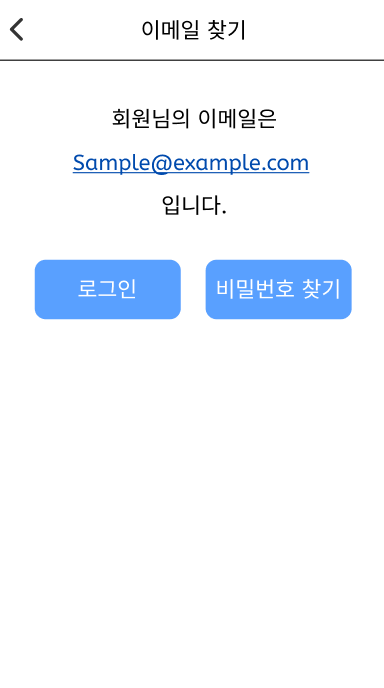
\includegraphics[width=0.27\textwidth]{img/D/6.png}
    \item Components Structure of Screen
    \begin{itemize}
        \item TopBar Component
        \item Text Component
        \begin{itemize}
            \item Displays property userEmail value.
        \end{itemize}
        \item Button Component
    \end{itemize}
    \item Flow of Screen
    \begin{itemize}
        \item Press the Go Back button to return to the previous Screen.
        \item Press the '로그인' button to go to the Login Screen.
        \item Press the '비밀번호 찾기’ button to go to the FindPw Screen.
        \\
    \end{itemize}
\end{itemize}
\newpage

\subsubsection{FindPw Screen}
\begin{itemize}
    \item[] 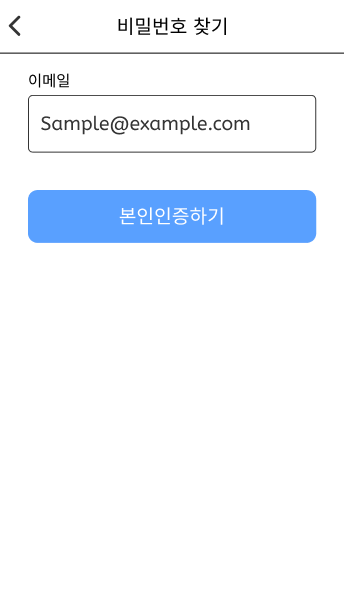
\includegraphics[width=0.27\textwidth]{img/D/7.png}
    \item Components Structure of Screen
    \begin{itemize}
        \item TopBar Component
        \item InputContainer Component
        \begin{itemize}
            \item On the FindPw screen, a checkEmail validation is performed, and the results are displayed below the input box.
        \end{itemize}
        \item Button Component
    \end{itemize}
    \item Flow of Screen
    \begin{itemize}
        \item Press the Go Back button to return to the previous Screen.
        \item Enter an email and press the '본인인증하기' button to call the FindPw API.
        \\
    \end{itemize}
\end{itemize}
\newpage

\subsubsection{HowToGoSpace Screen}
\begin{itemize}
    \item[] 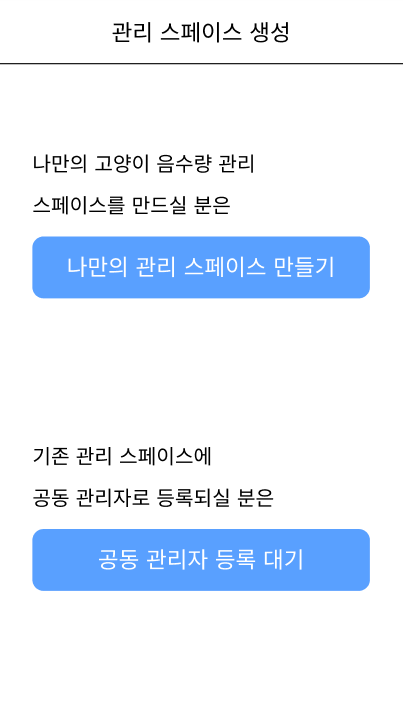
\includegraphics[width=0.27\textwidth]{img/D/8.png}
    \item Components Structure of Screen
    \begin{itemize}
        \item TopBar Component
        \begin{itemize}
            \item If there was a go-back button, the go-back button will not appear on the HowToGoSpace screen because it will be moved to the Start, Login screen while logged in.
        \end{itemize}
        \item Text Component
        \item Button Component
    \end{itemize}
    \item Flow of Screen
    \begin{itemize}
        \item Press the '나만의 관리 스페이스 만들기' button to go to the DeviceRegistration Screen.
        \item Press the '공동 관리자 등록 대기' button to go to the PendingCoManagerAddition Screen.
        \\
    \end{itemize}
\end{itemize}
\newpage

\subsubsection{PendingCoManagerAddition Screen}
\begin{itemize}
    \item[] 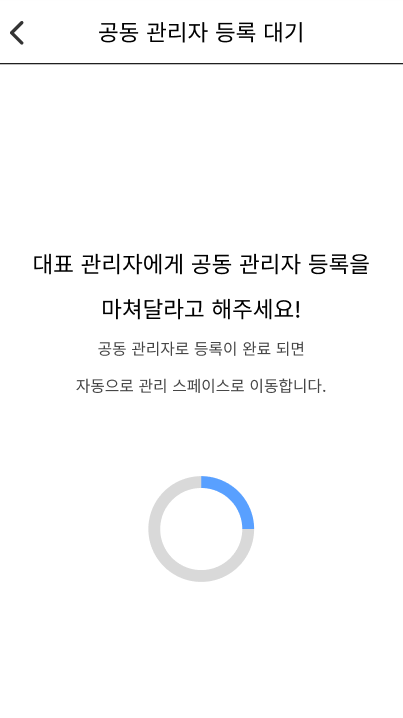
\includegraphics[width=0.27\textwidth]{img/D/9.png}
    \item Components Structure of Screen
    \begin{itemize}
        \item TopBar Component
        \item Text Component
        \item Loading Component
    \end{itemize}
    \item Flow of Screen
    \begin{itemize}
        \item Press the Back button to call the clearInterval function and return to the previous Screen.
        \item Use the setInterval function to call the GetManagementSpaceId API every 5 seconds until you are registered as a co-administrator.
        \\
    \end{itemize}
\end{itemize}
\newpage

\subsubsection{DeviceRegistration Screen}
\begin{itemize}
    \item[] 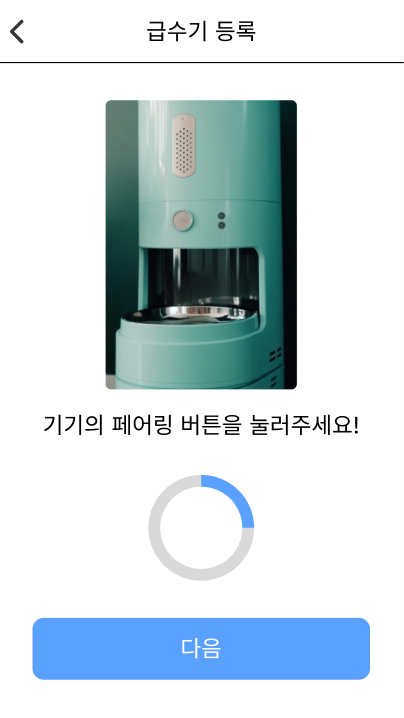
\includegraphics[width=0.27\textwidth]{img/D/10.png}
    \item Components Structure of Screen
    \begin{itemize}
        \item TopBar Component
        \item Image Component
        \item Text Component
        \item Loading Component
        \item Button Component
        \item DeviceSelect Component
        \item[] 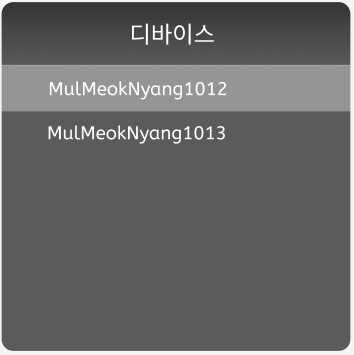
\includegraphics[width=0.2\textwidth]{img/D/10-1.png}
    \end{itemize}
    \item Flow of Screen
    \begin{itemize}
        \item Press the Back button to call the clearInterval function and return to the previous Screen.
    \end{itemize}
    \item Instead of Using API
    \begin{itemize}
        \item Since the device cannot actually be registered, it shows an animation during loading for 3 seconds, assuming that the pairing button is being pressed.
        \item Then, the Device Select Component is displayed and when the user selects Device, the property value of the Loading Component is changed to false and shows the pairing completed animation. Then it goes to the CatProfileRegistration Screen.
    \end{itemize}
\end{itemize}
\newpage

\subsubsection{CatProfileRegistration Screen}
\begin{itemize}
    \item[] 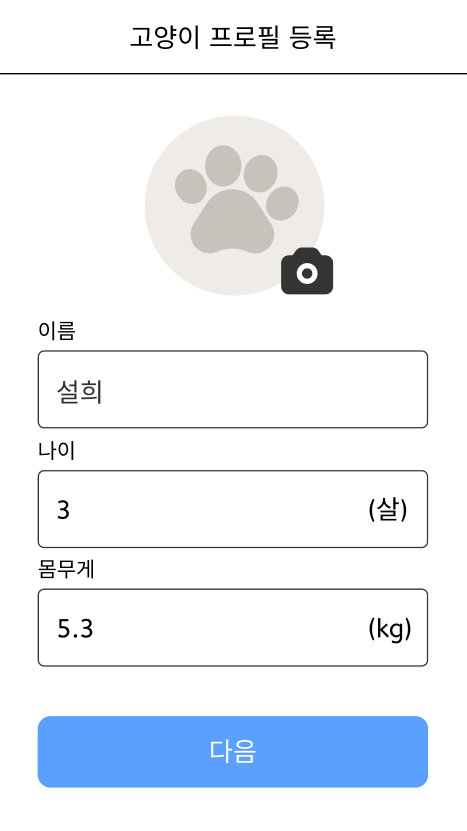
\includegraphics[width=0.27\textwidth]{img/D/11.png}
    \item Components Structure of Screen
    \begin{itemize}
        \item TopBar Component
        \item PhotoRegist Component
        \item InputContainer Component
        \begin{itemize}
            \item On the CatProfileRegistration screen, checkEmpty, checkNumber validation is performed, and the results of the check are displayed below the input box.
        \end{itemize}
        \item Button Component
    \end{itemize}
    \item Flow of Screen
    \begin{itemize}
        \item If the user does not have a management space yet, it displays Alert Component that says, "고양이 프로필을 최소한 한 마리 이상 등록 해야 관리 스페이스가 생성됩니다"
        \item Press the camera button to select a picture from the gallery, or take a picture with the camera to register a cat profile picture.
        \item Enter a name, age, and weight, and press the Next button to save the catName, catAge, and catWeight global variables with the Context API and moves to CatPhotosRegistration Screen.
    \end{itemize}
\end{itemize}
\newpage

\subsubsection{CatPhotosRegistration Screen}
\begin{itemize}
    \item[] 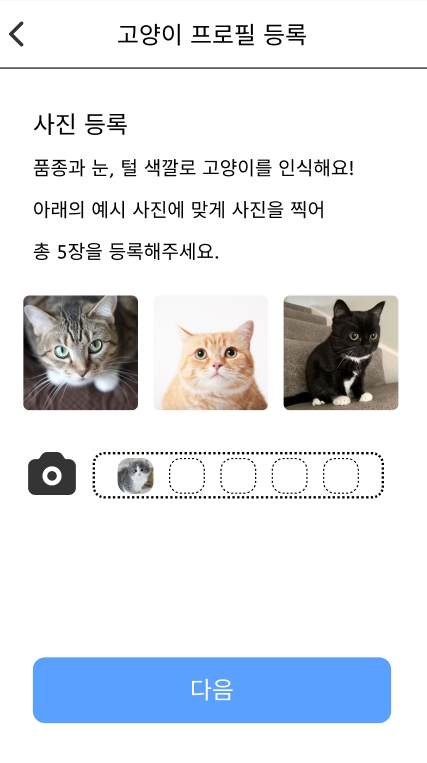
\includegraphics[width=0.27\textwidth]{img/D/12.png}
    \item Components Structure of Screen
    \begin{itemize}
        \item TopBar Component
        \item Text Component
        \item CatPhotosRegist Component
        \item Button Component
        \begin{itemize}
            \item User must register 5 photos to activate the button.
        \end{itemize}
    \end{itemize}
    \item Flow of Screen
    \begin{itemize}
        \item Press the camera button to select a picture from the gallery or take a picture with the camera to register a cat photo.
        \item Press the Go Back button to return to the previous Screen.
        \item Register 5 photos, press the 'Next' button to save the catPhotos global variable with the Context API and navigate to the CatFeedStuffRegistration Screen.
    \end{itemize}
\end{itemize}
\newpage

\subsubsection{CatFeedStuffRegistration Screen}
\begin{itemize}
    \item[] 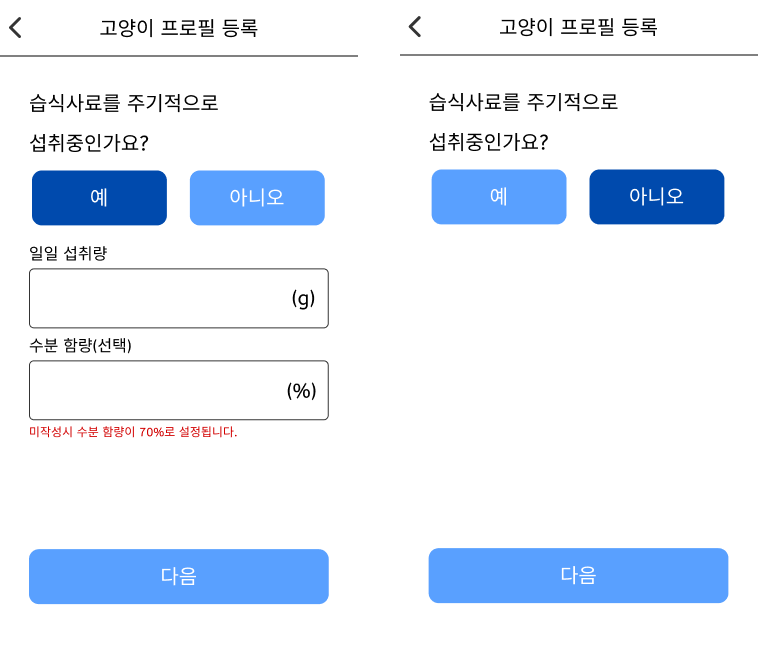
\includegraphics[width=0.45\textwidth]{img/D/13.png}
    \item Components Structure of Screen
    \begin{itemize}
        \item TopBar Component
        \item Text Component
        \item Button Component
        \begin{itemize}
            \item Press '예' to display the daily intake and water intake window.
        \end{itemize}
        \item InputContainer Component
        \begin{itemize}
            \item On the CatFeedStuffRegistration screen, checkEmpty, checkNumber validation is performed only when 'Yes' is pressed, and the results are displayed below the input box.
        \end{itemize}
    \end{itemize}
    \item Flow of Screen
    \begin{itemize}
        \item Press the Go Back button to return to the previous Screen.
        \item Press ‘예’ on the intake button and enter daily intake, water content. Then, press Next to save the catFeedStuffDailyConsumption, catFeedStuffMoistureContent global variables in the Context API.
        \item Press 'No' and then press 'Next' to store 0 in the catFeedStuffDailyConsumption, catFeedStuffMoistureContent global variable.
        \item Next, it goes to the CatHydrationRegistration Screen.
    \end{itemize}
\end{itemize}
\newpage

\subsubsection{CatHydrationRegistration Screen}
\begin{itemize}
    \item[] 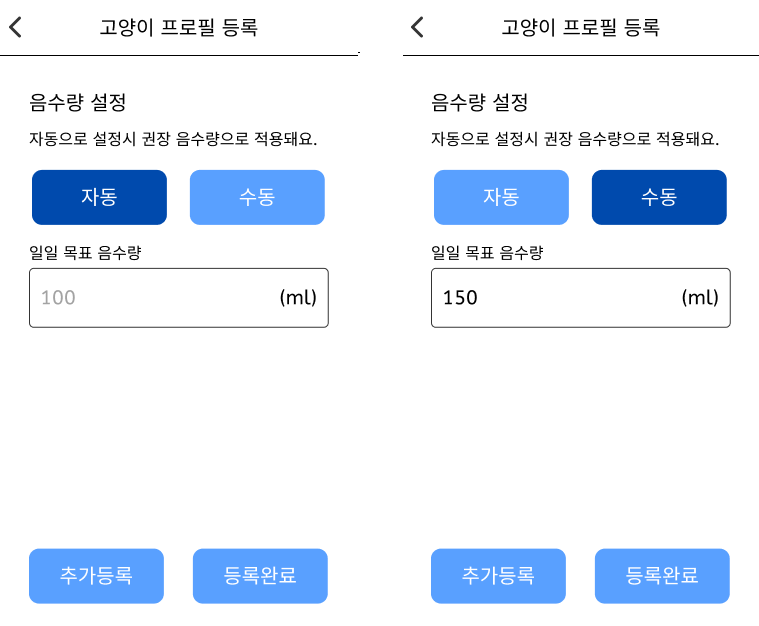
\includegraphics[width=0.45\textwidth]{img/D/14.png}
    \item Components Structure of Screen
    \begin{itemize}
        \item TopBar Component
        \item Text Component
        \item Button Component
        \item InputContainer Component
        \begin{itemize}
            \item Press 'Auto' to automatically calculate the recommended water intake and automatically enter it into the input box.
            \item On the CatHyditionRegistration screen, checkEmpty, checkNumber validation is performed, and the results of the inspection are displayed below the input box.
        \end{itemize}
    \end{itemize}
    \item Flow of Screen
    \begin{itemize}
        \item Press the Go Back button to return to the previous Screen.
        \item Press '자동' on how to set the water intake and then press the 'Additional Registration' or 'Registration Completed' button to store true in the isHyditionAuto global variable with the Context API and substitute the values of the global variable catFeedStuffDailyConsumption, catFeedStuffMoistureContent into the recommended drinking volume formula and store the calculated values in the catGoalHydition global variable.
        \item Press '수동' and enter the daily target water intake, then press the 'Additional Registration' or 'Registration Completed' button to store false in the global variable isHydrationAuto and save the input in the global variable catGoalHydration.
        \item Then, call the CatInfoRegist API.
        \item Once you have pressed the '추가 등록' button, it goes back to the CatProfileRegistration Screen.
        \item If you press the '등록 완료' button, delete the global variables' value related to cat information and navigate to the Main screen.
    \end{itemize}
\end{itemize}
\newpage

\subsubsection{Main Screen}
\begin{itemize}
    \item[] 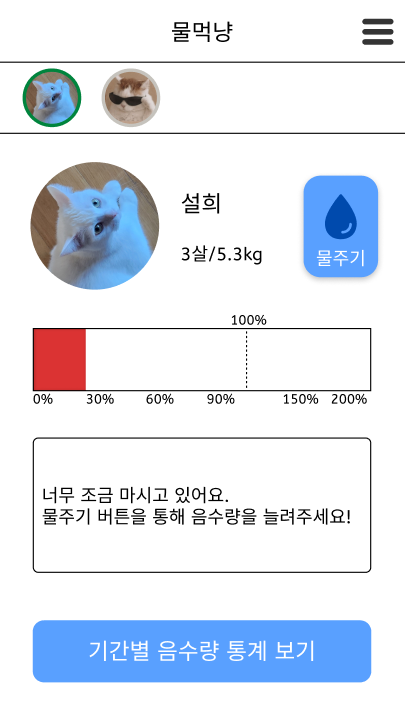
\includegraphics[width=0.27\textwidth]{img/D/15.png}
    \item Components Structure of Screen
    \begin{itemize}
        \item TopBar Component
        \item CatProfileList Component
        \item CatProfile Component
        \item HydrationButton Component
        \item HydrationGauge Component
        \begin{itemize}
            \item 0\% \~ 29\% : Red
            \item 30\% \~ 59\% : Yellow
            \item 60\% \~ 89\% : Green
            \item 90\% \~ 149\% : Blue
            \item 150\% \~ 200\% : Red
        \end{itemize}
        \item EvaluationText Component
        \item Button Component
    \end{itemize}
    \item Flow of Screen
    \begin{itemize}
        \item Call the GetCatProfileList API in the Mount step, process the response, and call the GetCatMainInfo API.
        \item Press the menu button to open the Drawer.
        \item In the cat profile list at the top, call the GetCatMainInfo API whenever user press a picture of another cat profile that is not currently selected.
        \item When you press the '물주기' button, a cat-calling sound comes out from the built-in speaker, and water comes out when the cat approaches the water supply.
        \item You will receive a push notification whether the cat drank water or not within 10 minutes.
        \item A water intake gauge shows how much the cat has intaken today so far.
        \item Different assessments appear depending on the gauge.
        \item Press the '기간별 음수량 통계 보기' button to go to the Hydration Statistics Screen.
    \end{itemize}
\end{itemize}
\newpage

\subsubsection{HydrationStatistics Screen}
\begin{itemize}
    \item[] 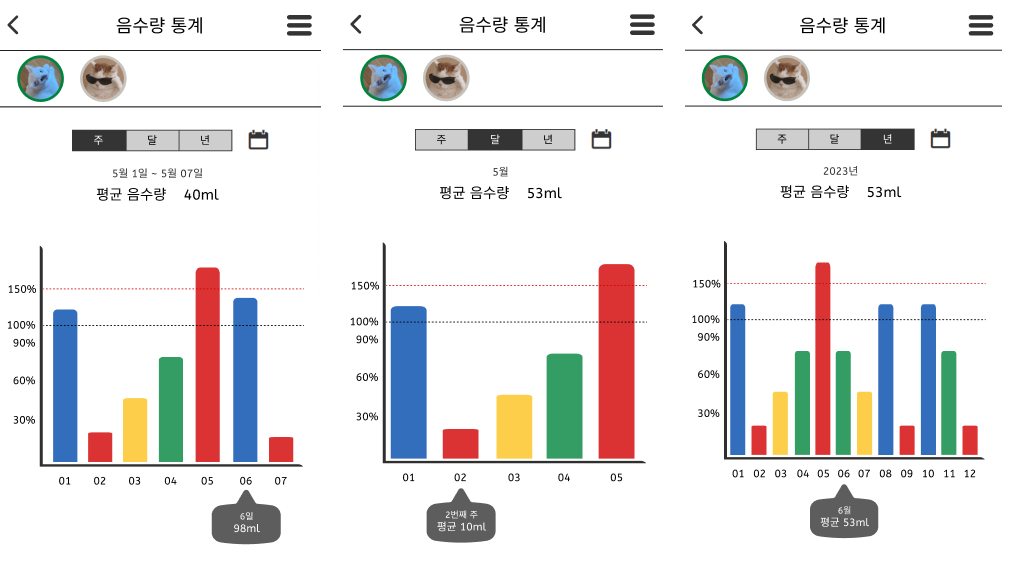
\includegraphics[width=0.47\textwidth]{img/D/16.png}
    \item Components Structure of Screen
    \begin{itemize}
        \item TopBar Component
        \item CatProfileList Component
        \item RangeSet Component
        \item Calender Component
        \item[] 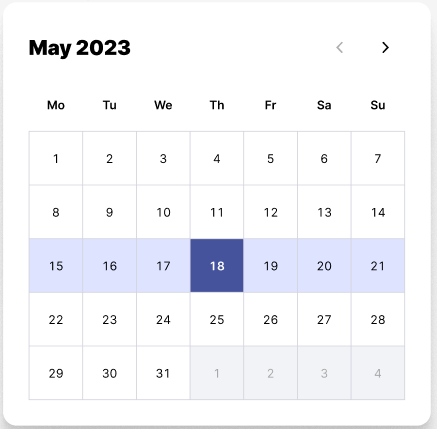
\includegraphics[width=0.2\textwidth]{img/D/16-1.png}
        \item AvgText Component
        \item BarGraph Component
        \begin{itemize}
            \item Bar Component
            \item BarDetail Component
        \end{itemize}
    \end{itemize}
    \item Flow of Screen
    \begin{itemize}
        \item GetCatStatistics API is called in the Mount step.
        \item Press the Go Back button to return to the previous Screen.
        \item Press the menu button to open the Drawer.
        \item From the cat profile list at the top, whenever you click cat's picture that is not currently selected, change the statistical period, or select a specific week/month/year in the calendar, GetCatStatistics API is called.
        \item For '주', if you select a specific date in the calendar, the week containing that date is selected.
        \item Touch a particular bar to display detailed water intake amount.
    \end{itemize}
\end{itemize}
\newpage

\subsubsection{Drawer}
\begin{itemize}
    \item[] 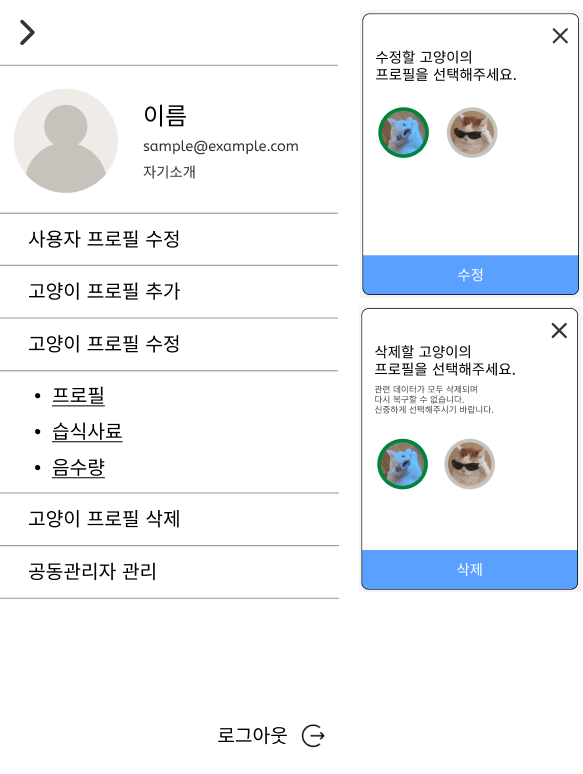
\includegraphics[width=0.33\textwidth]{img/D/17.png}
    \item Components Structure of Screen
    \begin{itemize}
        \item TopBar Component
        \item UserProfile Component
        \item TextContainerButton Component
        \begin{itemize}
            \item For users with only one cat registered, the Delete Cat Profile button does not appear.
        \end{itemize}
        \item UnderlineTextButton Component
        \item LogoutButton Component
        \item LongAlert Component
        \begin{itemize}
            \item IconButton Component
            \item Title Component
            \item Text Component
            \item CatProfileList Component
            \item Button Component
        \end{itemize}
    \end{itemize}
    \item Flow of Screen
    \begin{itemize}
        \item Press the Close button to close the Drawer.
        \item Press the '사용자 프로필 수정' button to go to the UserProfileModification Screen.
        \item Pressing the '프로필', '습식사료', and '음수량' buttons under '고양이 프로필 수정' displays LongAlert Component to select the cat to modify the information.
        \item Select the cat you want to modify and press the '수정' button to go to the Cat\_\_\_\_\_Modification Screen.
        \item When you press the 'Delete Cat Profile' button, a LongAlert Component will appear to select the cat to delete all the information.
        \item Select the cat you want to delete and press the '삭제' button to call the DeleteCatInfo API.
        \item Press the '공동관리자 관리' button to navigate to the CoManagerSet Screen.
        \item If user presses the Logout button, the Alert Component that says 'Do you really want to log out?' apeears and when user proceed with 'Yes', the Logout API is called.
    \end{itemize}
\end{itemize}
\newpage

\subsubsection{UserProfileModification Screen}
\begin{itemize}
    \item[] 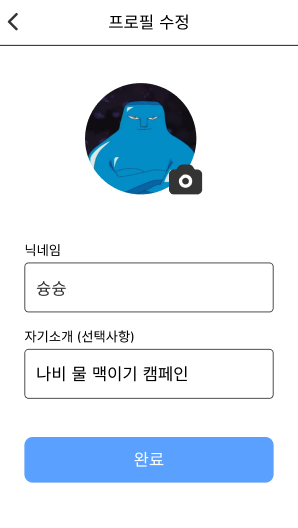
\includegraphics[width=0.27\textwidth]{img/D/18.png}
    \item Components Structure of Screen
    \begin{itemize}
        \item Identical to UserProfileRegistration Screen.
    \end{itemize}
    \item Flow of Screen
    \begin{itemize}
        \item Call the GetUserProfile API in the Mount step.
        \item Call the ModifyUserProfile API when the '완료' button is pressed.
        \item The rest is the same as the UserProfileRegistration Screen.
    \end{itemize}
\end{itemize}
\newpage

\subsubsection{CatProfileModification Screen}
\begin{itemize}
    \item[] 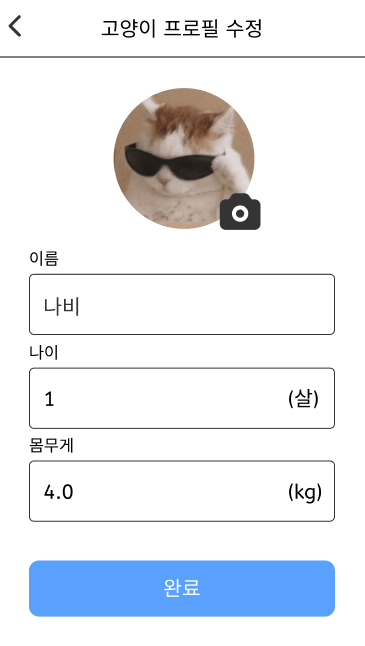
\includegraphics[width=0.27\textwidth]{img/D/19.png}
    \item Components Structure of Screen
    \begin{itemize}
        \item Identical to CatProfileRegistration Screen.
    \end{itemize}
    \item Flow of Screen
    \begin{itemize}
        \item Call the GetCatProfile API in the Mount step.
        \item Call the ModifyUserProfile API when the '완료' button is pressed.
        \item The rest is the same as the CatProfileRegistration Screen.
    \end{itemize}
\end{itemize}
\newpage

\subsubsection{CatFeedStuffModification Screen}
\begin{itemize}
    \item[] 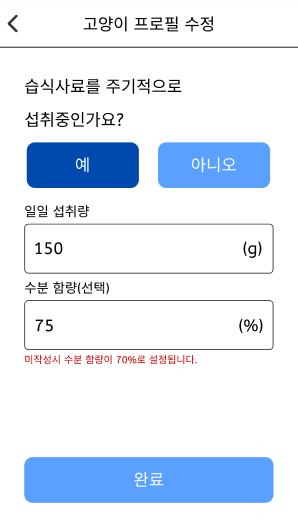
\includegraphics[width=0.27\textwidth]{img/D/20.png}
    \item Components Structure of Screen
    \begin{itemize}
        \item Identical to CatFeedStuffRegistration Screen.
    \end{itemize}
    \item Flow of Screen
    \begin{itemize}
        \item Call the GetCatFeedStuffAPI in the Mount step.
        \item Call the ModifyCatFeedStuff API when the '완료' button is pressed.
        \item The rest is the same as the CatFeedStuffRegistration Screen.
    \end{itemize}
\end{itemize}
\newpage

\subsubsection{CatHydrationModification Screen}
\begin{itemize}
    \item[] 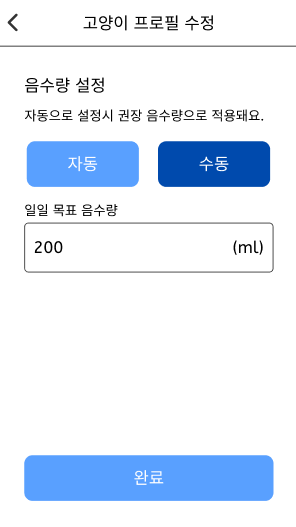
\includegraphics[width=0.27\textwidth]{img/D/21.png}
    \item Components Structure of Screen
    \begin{itemize}
        \item Identical to CatHydrationRegistration Screen.
    \end{itemize}
    \item Flow of Screen
    \begin{itemize}
        \item Call the GetCatHydration in the Mount step.
        \item Call the ModifyCatHydration API when the '완료' button is pressed.
        \item The rest is the same as the CatHydrationRegistration Screen.
    \end{itemize}
\end{itemize}
\newpage

\subsubsection{CoManagerSet Screen}
\begin{itemize}
    \item[] 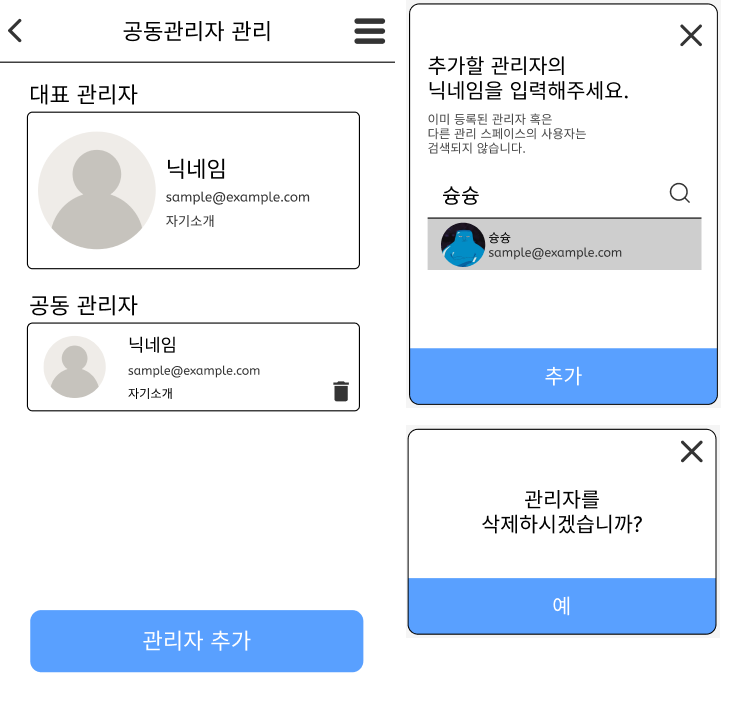
\includegraphics[width=0.47\textwidth]{img/D/22.png}
    \item Components Structure of Screen
    \begin{itemize}
        \item TopBar Component
        \item MainManagerCard Component
        \item CoManagersCardList Component
        \begin{itemize}
            \item CoManagerCard Component
        \end{itemize}
        \item Button Component
        \item LongAlert Component
        \begin{itemize}
            \item IconButton Component
            \item Title Component
            \item Text Component
            \item Search Component
            \item SearchedUser Component
            \item Button Component
        \end{itemize}
    \end{itemize}
    \item Flow of Screen
    \begin{itemize}
        \item Call the GetManagerList API in the Mount step.
        \item Pressing the Add Administrator button to displays the LongAlert Component. After entering a nickname and when you press the search icon, it calls the UserSearch API.
        \item Select the administrator user wants to add and press the Add button to call the AddCoManager API.
        \item On the Administrator Screen, the Trash icon appears in the Co Manager Card, and when you press the '예’' button in the Manager Delete Alert Component, the DeleteCoManager API is called.
        \\
    \end{itemize}
\end{itemize}

\subsection{API Usage Logic}
\subsubsection{AutoLogin API}
\begin{itemize}
    \item Client send HTTP Request to Server
    \begin{itemize}
        \item Case 1) Users with auto login disabled
        \begin{itemize}
            \item Set the userEmail value to HTTP Request and send the Request to the Server.
        \end{itemize}
        \item Case 2) Users with auto login enabled
        \begin{itemize}
            \item Set the cookie that contains the Session ID in the React Native app storage to HTTP Request and send the request to the Server.
            \\
        \end{itemize}
    \end{itemize}
    \item HTTP Request process in the sever, HTTP Response from server to client
    \begin{itemize}
        \item Case 1) Users with auto login disabled
        \begin{itemize}
            \item If the value set in the HTTP Request is userEmail, create a session and add a record along with userEmail to the session table.
            \item Configure Session ID and generate a cookie.
            \item When querying the record in the user table with userEmail, if there is a value for management\_space\_id, it is saved in the variable managementSpaceId, and if not, it is saved as null.
            \item Set userEmail, managementSpaceId, and Cookie in HTTP Response to send a response to the Client.
        \end{itemize}
        \item Case 2) Users with auto login enabled
        \begin{itemize}
            \item The session ID stored in the cookie set in the HTTP Request inquires the record in the session table and stores the user\_email value in the userEmail variable.
            \item When querying the record in the user table with userEmail, if there is a value for management\_space\_id, it is saved in the variable managementSpaceId, and if not, it is saved as null.
            \item Set userEmail, managementSpaceId to HTTP Response and send a response to the Client.
            \\
        \end{itemize}
    \end{itemize}
    \item HTTP Response Processing in Client side
    \begin{itemize}
        \item The userEmail value set in the HTTP Response is stored as a global variable userEmail using the Context API, and if the managementSpaceId value is not null, it is also stored as a global variable managementSpaceId.
        \item If the cookie is set in HTTP Response, it saves the cookie in the React Native App storage before moving into the screen.
        \item If the user have a managementSpaceId value, go to the Main screen, and if the value is null, go to the HowToGoSpace screen.
        \\
    \end{itemize}
\end{itemize}

\subsubsection{QuickSignUp APIs : NaverSignUp, KaKaoSignUp, GoogleSignUp}
\begin{itemize}
    \item HTTP Response for Server → Client
    \begin{itemize}
        \item Using Naver, Kakao, and Google's simple login APIs and with the user profile information provided, userEmail values are first stored in variables.
        \item Check the record in the user table with the userEmail value, store true in the userExists variable if there is a registered user, and store false if not.
        \item Case 1) Registered Users → Easy Login
        \begin{itemize}
            \itemIf the userExists value is true, check the record in the user table with the userEmail value, and if there are user\_nickname and management\_space\_id values, store them in the userNickname and managementSpaceId variables, and if not, store null.
            \item When login is successful, store true to the variable loginSuccess.
            \item Set loginSucess, userEmail, userNickname, managementSpaceId to HTTP Response and send it to the Client.
        \end{itemize}
        \item Case 2) Unregistered users → Easy membership registration
        \begin{itemize}
            \item If the userExists value is false, the remaining profile information is also stored in the variable, and add record containing userEmail, userPw, userName, and userPhoneNum values to the user table.
            \item When registeration is successful, store true to the variable registerSuccess
            \item Set registerSuccess, userEmail to HTTP Response and send it to Client.
            \\
        \end{itemize}
    \end{itemize}
    \item HTTP Response Processing in Client side
    \begin{itemize}
        \item The userEmail value set in HTTP Response is stored as a global variable userEmail using the Context API.
        \item Case 1) Registered Users → Easy Login
        \begin{itemize}
            \item If loginSuccess is set in HTTP Response, check whether there is a value stored in userNickname or null is stored.
            \item The existence of the userNickname value means that the user profile has been registered.
            \item Case 1-1) Users that have profile registration completed
            \begin{itemize}
                \item Display an Alert Component that says, ‘자동 로그인을 설정하시겠습니까?’.
                \item If '예', follow case 1-1-1 below.
                \item Then, if the managementSpaceId value set in HTTP Response is not null, it is stored as a global variable managementSpaceId using the Context API.
                \item If the user have a managementSpaceId value, go to the Main screen, and if the value is null, go to the HowToGoSpace screen.
                \item Case 1-1-1) User who wants auto login
                \begin{itemize}
                    \item Set the userEmail value to HTTP Request and send the request to the Auto Login API in the server.
                    \item This corresponds to Case 1 of the AutoLogin API.
                    \item Store the cookie set in the HTTP Response sent from the AutoLogin API in the React Native App Storage.
                \end{itemize}
            \end{itemize}
            \begin{itemize}
                \item Case 1-2) User who needs to register for a user profile
                \begin{itemize}
                    \item If the userNickname value is null, go to the UserProfileRegistration screen.
                \end{itemize}
            \end{itemize}
        \end{itemize}
        \item Case 2) Unregistered users → Easy membership registration
        \begin{itemize}
            \item If registerSuccess is set in HTTP Response, go to the UserProfileRegistration screen.
            \\
        \end{itemize}
    \end{itemize}
\end{itemize}

\subsubsection{Login API}
\begin{itemize}
    \item HTTP Request From Client to Server
    \begin{itemize}
        \item Set userEmail, userPw, and autoLogin values to HTTP Request and send a request to the server.
        \\
    \end{itemize}
    \item HTTP requests process in Server, HTTP Response from Server to Client
    \begin{itemize}
        \item Case 1) Registered User
        \begin{itemize}
            \item With the userEmail and userPw values set in the HTTP Request, look up the record in the user table. If there is a registered user, store true in the userExists variable and if not, store false.
            \item If the record has user\_nickname and management\_space\_id values, store them in the userNickname and managementSpaceId variables, respectively, and if not, store null.
            \item Case 1-1) Who checked the Auto Login check box
            \begin{itemize}
                \item If the userExists value is true and the AutoLogin value set in the HTTP Request is also true, the userEmail value is set in the HTTP Request and the request is sent to the AutoLogin API.
                \item This corresponds to Case 1 of the Auto Login API.
                \item The cookie set in the HTTP Response transmitted from the Auto Login API is stored in the variable.
                \item Set userEmail, userNickname, managementSpaceId, and Cookie in HTTP Response to send a response to the Client.
            \end{itemize}
            \item Case 1-2) Users who did not check the Auto Login check box
            \begin{itemize}
                \item If the AutoLogin value set in the HTTP Request is false, set userEmail, userNickname, and managementSpaceId to HTTP Response and send a response to the Client.
            \end{itemize}
        \end{itemize}
    \end{itemize}
    \begin{itemize}
        \item Case 2) Unregistered User
        \begin{itemize}
            \item If the userExists value is false, set the userExists value to HTTP Response and send a response to the Client.
            \\
        \end{itemize}
    \end{itemize}
    \item HTTP Response process in Client side
    \begin{itemize}
        \item Case 1) Registered User
        \begin{itemize}
            \item If userEmail is set in HTTP Response, the userEmail value is saved as a global variable userEmail using the Context API.
            \item Check whether there is a set userNickname value in HTTP Response or null.
            \item The existence of the userNickname value means that the user profile has been registered.
            \item Case 1-1) User that has completed profile registration
            \begin{itemize}
                \item If the managementSpaceId value set in HTTP Response is not null, it is stored as a global variable managementSpaceId.
                \item If the cookie is set in HTTP Response, store the cookie in the React Native App storage.
                \item Then, if the user has a managementSpaceId value, it moves to the Main screen, and if the value is null, it moves to the HowToGoSpace screen.
            \end{itemize}
            \item Case 1-2) User who needs to register user profile
            \begin{itemize}
                \item If the userNickname value is null, display an Alert Component that says "자동 로그인 설정은 사용자 프로필 등록을 한 다음 사용이 가능합니다." and navigate to the UserProfileRegistration screen.
            \end{itemize}
        \end{itemize}
        \item Case 2) Unregistered User
        \begin{itemize}
            \item If the userExists value set in HTTP Response is false, it displays an Alert Component that says "해당되는 사용자가 없습니다." and keeps the Login screen.
            \\
        \end{itemize}
    \end{itemize}
\end{itemize}

% \subsubsection{NICEAuth API}
% \begin{itemize}
%     \item Server → Client로 HTTP Response
%     \begin{itemize}
%         \item NICE의 휴대폰 본인인증 API를 사용한다.
%         \item Case 1) 본인인증 완료
%         \begin{itemize}
%             \item 본인 인증 완료 후 사용자의 정보를 제공 받아, 그 중 userName, userPhoneNum 값을 변수에 저장한다.
%             \item 본인 인증에 성공했음을 true로 변수 sucessAuth에 저장한다.
%             \item sucessAuth, userName, userPhonenum을 HTTP Response에 설정하여 Client에 전송한다.
%         \end{itemize}
%         \item Case 2) 본인인증 실패
%         \begin{itemize}
%             \item 만약 본인 인증을 중도에 그만뒀다면, sucessAuth에 false를 저장한다.
%             \item sucessAuth를 HTTP Response에 설정하여 Client에 전송한다.
%             \\
%         \end{itemize}
%     \end{itemize}
% \end{itemize}

\subsubsection{LocalSignUp API}
\begin{itemize}
    \item HTTP Request from Client to Server 
    \begin{itemize}
        \item Set the userEmail, userPw value to HTTP Request and send the request to the server.
        \\
    \end{itemize}
    \item HTTP Request Process in Server side, HTTP Response from Server to Client 
    \begin{itemize}
        \item Retrieve a record from the user table using the userEmail value set in the HTTP Request. If a registered user exists, store true in the userExists variable; otherwise, store false.
        \item Case 1) Registered User
        \begin{itemize}
            \item If the userExists value is true, set userExists in the HTTP Response and send the response to the client.
        \end{itemize}
        \item Case 2) Unregistered User
        \begin{itemize}
            \item If the userExists value is false, store the userEmail and userPw set in the HTTP Request in variables.
            % NICE AUth Part. Comment out?
            \item Next, send a request to the NICE Auth API to proceed with identity verification.
            \begin{itemize}
                \item Case 2-1) Identity Verification Completed
                \begin{itemize}
                    \item If the successAuth in the HTTP Response sent by the NICE Auth API is true, add a record to the user table with the userName and userPhonenum values along with the userEmail and userPw variables.
                    \item Store true in the stepOneDone variable.
                \end{itemize}
                \item Case 2-2) Identity Verification Failed
                \begin{itemize}
                    \item If the successAuth in the HTTP Response sent by the NICE Auth API is false, store false in the stepOneDone variable.
                \end{itemize}
                \item Set stepOneDone and userEmail in the HTTP Response and send the response to the client.
                \\
            \end{itemize}
        \end{itemize}
    \end{itemize}
    \item Client-side HTTP Response Handling
    \begin{itemize}
        \item Case 1) Registered User
        \begin{itemize}
            \item If the HTTP Response has userExists set, display an Alert Component with the message "이미 회원 가입된 이메일입니다." and navigate to the Login screen.
        \end{itemize}
        \item Case 2) Unregistered User
        \begin{itemize}
            \item Case 2-1) Identity Verification Completed
            \begin{itemize}
                \item If the stepOneDone value in the HTTP Response is true, save the userEmail value as a global variable using Context API and navigate to the UserProfileRegistration screen.
            \end{itemize}
            \item Case 2-2) Identity Verification Failed
            \begin{itemize}
                \item If the stepOneDone value in the HTTP Response is false, display an Alert Component with the message "본인 인증에 실패하셨습니다." and stay on the LocalSignUp screen.
                \\
            \end{itemize}
        \end{itemize}
    \end{itemize}
\end{itemize}

\subsubsection{RegistUserProfile API}
\begin{itemize}
    \item Client → Server HTTP Request
    \begin{itemize}
        \item Send userProfilePhoto, userNickname, userIntroduction values, along with the userEmail stored as a global variable, in the HTTP Request from the Client to the Server.
        \\
    \end{itemize}
    \item Server-side HTTP Request Handling, Server → Client HTTP Response
    \begin{itemize}
        \item Retrieve a record from the user table using the userNickname value set in the HTTP Request. If the nickname already exists, store true in the nicknameExists variable.
        \item Case 1) Duplicate Nickname
        \begin{itemize}
            \item If nicknameExists is true, set nicknameExists in the HTTP Response and send it to the Client.
        \end{itemize}
        \item Case 2) Non-duplicate Nickname
        \begin{itemize}
            \item If nicknameExists is false, retrieve a record from the user table using the userEmail value set in the HTTP Request, and add userProfilePhoto, userNickname, and userIntroduction values.
            \item Save true in the stepTwoDone variable.
            \item Set stepTwoDone in the HTTP Response and send it to the Client.
            \\
        \end{itemize}
    \end{itemize}
    \item Client-side HTTP Response Handling
    \begin{itemize}
        \item Case 1) Duplicate Nickname
        \begin{itemize}
            \item If the HTTP Response has nicknameExists set to true, display an Alert Component with the message "이미 존재하는 닉네임입니다." and stay on the UserProfileRegistration screen.
        \end{itemize}
        \item Case 2) Non-duplicate Nickname
        \begin{itemize}
            \item If the HTTP Response has stepTwoDone set, display an Alert Component with the message "사용자 프로필 등록이 완료되었습니다. 자동 로그인을 설정하시겠습니까??".
            \item If the user selects ‘예’ follow the instructions in case 2-1.
            \item Then, navigate to HowToGoSpace Screen.
            \item Case 2-1) User Who Wants Automatic Login
            \begin{itemize}
                \item Set the userEmail value in the HTTP Request and send a request to the Auto Login API on the Server. 
                \item This corresponds to Case 1 in the Auto Login API.
                \item Store the Cookie received from the HTTP Response of the Auto Login API in the React Native App's storage.
                \\
            \end{itemize}
        \end{itemize}
    \end{itemize}
\end{itemize}

% \subsubsection{FindEmail API}
% \begin{itemize}
%     \item Client → Server로 HTTP Request
%     \begin{itemize}
%         \item userName, userPhoneNum 값을 HTTP Request에 설정하여 Server에 Request를 전송한다.
%         \\
%     \end{itemize}
%     \item Server에서 HTTP Request 처리, Server → Client로 HTTP Response
%     \begin{itemize}
%         \item HTTP Request에 설정된 userName, userPhoneNum 값으로 user table에서 record를 조회해, 등록된 사용자가 존재한다면, user\_email 값을 변수 userEmail에 저장한다.
%         \item 등록된 사용자가 존재하지 않는다면, userExists 변수에 false 값을 저장한다. 
%         \item Case 1) 등록된 사용자
%         \begin{itemize}
%             \item userEmail을 HTTP Response에 설정하여 Client에 Response를 전송한다.
%         \end{itemize}
%         \item Case 2) 등록되지 않은 사용자
%         \begin{itemize}
%             \item userExists를 HTTP Response에 설정하여 Client에 Response를 전송한다.
%             \\
%         \end{itemize}
%     \end{itemize}
%     \item Client에서 HTTP Response 처리, Data Binding
%     \begin{itemize}
%         \item Case 1) 등록된 사용자
%         \begin{itemize}
%             \item HTTP Response에 userEmail이 설정되어 있다면, userEmail 값을 property로 전달하여 FindEmailResult 화면으로 이동하고, 사용자에게 이메일을 알려준다.
%         \end{itemize}
%         \item Case 2) 등록되지 않은 사용자
%         \begin{itemize}
%             \item HTTP Response에 설정된 userExists 값이 false라면, ‘해당되는 사용자가 없습니다.’ 라고 쓰인 Alert Component를 띄우고, FindEmail 화면을 유지한다.
%             \\
%         \end{itemize}
%     \end{itemize}
% \end{itemize}

\subsubsection{FindPw API}
\begin{itemize}
    \item Client → Server HTTP Request
    \begin{itemize}
        \item userEmail 값을 HTTP Request에 설정하여 Server에 Request를 전송한다.
        \item Set userEmail value in the HTTP Request and send Request to the Server.
        \\
    \end{itemize}
    \item Server-side HTTP Request Handling, Server → Client HTTP Response
    \begin{itemize}
        \item Retrieve a record from the user table using the userEmail value set in the HTTP Request. If a registered user exists, store true in the userExists variable; otherwise, store false.
        \item Case 1) Registered User
        \begin{itemize}
            \item If userExists is true, send a request to the NICE Auth API for identity verification.
            \item Case 1-1) Identity Verification Completed
            \begin{itemize}
                \item If the successAuth in the HTTP Response received from the NICE Auth API is true, retrieve the user\_pw from the user table using userName and userEmail, and store it in the userPw variable.
                \item Use the express-email package to send the userPw to the user's email.
                \item Once the email has been sent, store true in the sendMail variable.
                \item Set sendMail in the HTTP Response and send it to the client.
            \end{itemize}
            \item Case 1-2) Identity Verification Failed
            \begin{itemize}
                \item If the successAuth in the HTTP Response from the NICE Auth API is false, set successAuth in the HTTP Response and send it to the client.
            \end{itemize}
        \end{itemize}
        \item Case 2) Unregistered User
        \begin{itemize}
            \item If userExists is false, set userExists in the HTTP Response and send the response to the client.
            \\
        \end{itemize}
    \end{itemize}
    \item Client-side HTTP Response Handling
    \begin{itemize}
        \item Case 1) Registered User
        \begin{itemize}
            \item Case 1-1) Identity Verification Completed
            \begin{itemize}
                \item If the HTTP Response has sendMail set, display an Alert Component with the message "비밀번호가 이메일로 전송되었습니다" and navigate to the Login screen.
            \end{itemize}
            \item Case 1-2) Identity Verification Failed
            \begin{itemize}
                \item If the successAuth value in the HTTP Response is false, display an Alert Component with the message "본인 인증에 실패하셨습니다." and stay on the FindPw screen.
            \end{itemize}
        \end{itemize}
        \item Case 2) Unregistered User
        \begin{itemize}
            \item If the userExists value in the HTTP Response is false, display an Alert Component with the message "회원 가입된 이메일이 아닙니다." and stay on the FindPw screen.
            \\
        \end{itemize}
    \end{itemize}
\end{itemize}

% \subsubsection{GetManagementSpaceId API}
% \begin{itemize}
%     \item Client → Server로 HTTP Request
%     \begin{itemize}
%         \item 전역 변수로 저장된 userEmail 값을 HTTP Request에 설정하여 Server에 Request를 전송한다.
%         \\
%     \end{itemize}
%     \item Server에서 HTTP Request 처리, Server → Client로 HTTP Response
%     \begin{itemize}
%         \item HTTP Request에 설정된 userEmail 값으로 user table에서 record를 조회해, management\_space\_id 값을 변수 managementSpaceId에 저장한다.
%         \item managementSpaceId를 HTTP Response에 에 설정하여 Client에 Response를 전송한다.
%         \\
%     \end{itemize}
%     \item Client에서 HTTP Response 처리, Data Binding
%     \begin{itemize}
%         \item HTTP Response에 managementSpaceId가 설정되어 있는 게 확인이 된다면, cleartInterval 함수를 호출하고 Loading Component의 property 값을 false로 바꿔 등록 완료 애니메이션을 보여준 뒤, Main 화면으로 이동한다.
%         \\
%     \end{itemize}
% \end{itemize}

\subsubsection{RegistCatInfo API}
\begin{itemize}
    \item Client → Server HTTP Request
    \begin{itemize}
        \item Case 1) First-time Cat Registration (For users with no existing management space):
        \begin{itemize}
            \item Send the userEmail, catProfilePhoto, catName, catAge, catWeight, catPhotos, catFeedStuffDailyConsumption, catFeedStuffMoistureContent, isHydrationAuto, and catGoalHydration values that are saved from global variables in the HTTP Request to the Server.
        \end{itemize}
        \item Case 2) Additional Cat Registration (For users with an existing management space):
        \begin{itemize}
            \item Include the managementSpaceId value from global variables in the HTTP Request and send it to the Server.
            \\
        \end{itemize}
    \end{itemize}
    \item Server-side HTTP Request Handling, Server → Client HTTP Response
    \begin{itemize}
        \item Case 1) First-time Cat Registration (For users with no existing management space):
        \begin{itemize}
            \item Step 1) If the managementSpaceId is not set in the HTTP Request, generate a 10-digit random value using the Math.random() method and store it in the spaceId variable.
            \item Step 2) ynamically create the management\_space\_\$\{spaceId\} table.
            \item Step 3) Add a record with spaceId and the userEmail value from the HTTP Request.
            \item Step 4) Dynamically create cat\_in\_management\_\$\{spaceId\} table.
            \item (common) Step 5) Add records to the cat\_in\_management\_\$\{spaceId\} table with the values of cat information from the HTTP Request.
            \item (common) Step 6) Retrieve the cat\_id from cat\_in\_management\_\$\{spaceId\} table based on the catName value from the HTTP Request and store it in the catId variable.
            \item Step 7) Dynamically create cat\_hydration\_statistics\_\$\{catId\} table.
            \item (common) Step 8) Add a record to the cat\_hydration\_statistics\_\$\{catId\} table with the value of catGoalHydration from the HTTP Request.
            \item Step 9) Add the spaceId value to the management\_space\_id column in the user table based on the retrieved information, userEmail.
            \item Step 10) Set spaceId in the HTTP Response and send it to the Client.
        \end{itemize}
        \item Case 2) Additional Cat Registration (For users with an existing management space):
        \begin{itemize}
            \item Step 1) If the managementSpaceId is set in the HTTP Request, store it in the spaceId variable.
            \item (common) Step 2) Add records to the cat\_in\_management\_\$\{spaceId\} table with the values of cat information from the HTTP Request.
            \item (common) Step 3) Retrieve the cat\_id from the cat\_in\_management\_\$\{spaceId\} table based on the catName value from the HTTP Request and store it in the catId variable.
            \item (common) Step 4) Add a record to the cat\_hydration\_statistics\_\$\{catId\} table with the value of catGoalHydration from the HTTP Request.
            \item Step 5) Store true in the addCatInfo variable and set addCatInfo in the HTTP Response to send it to the Client.
            \\
        \end{itemize}
    \end{itemize}
    \item Client-side HTTP Response Handling
    \begin{itemize}
        \item Case 1) First-time Cat Registration (For users with no existing management space):
        \begin{itemize}
            \item If spaceId is set in the HTTP Response, store it as the managementSpaceId global variable using the Context API.
            \\
        \end{itemize}
    \end{itemize}
\end{itemize}

\subsubsection{GetCatProfileList API}
\begin{itemize}
    \item Client → Server HTTP Request
    \begin{itemize}
        \item Send the managementSpaceId value from the global variables in the HTTP Request to the Server.
        \\
    \end{itemize}
    \item Server-side HTTP Request Handling, Server → Client HTTP Response
    \begin{itemize}
        \item Store the managementSpaceId value from the HTTP Request in the spaceId variable.
        \item Query the cat\_id values from the cat\_in\_management\_space\_\$\{spaceId\} table and store them in the catIdArr array variable.
        \item Retrieve the cat\_profile\_photo values only from cat\_in\_management\_space\_\$\{spaceId\} table and store them in the catProfilePhotoArr array variable.
        \item Set the catIdArr and catProfilePhotoArr arrays in the HTTP Response to send them to the Client.
        \\
    \end{itemize}
    \item Client-side HTTP Response Handling, Data Binding
    \begin{itemize}
        \item Store the catIdArr and catProfilePhotoArr arrays set in the HTTP Response as global variables using the Context API.
        \item Inside the Cat Profile List Component, use the map method to display Cat Profile List Components. Pass the key prop as 'i,' catId prop as catIdArr[i], and catProfilePhoto prop as catProfilePhotoArr[i].
        \item Set the onFocus prop of the Cat Profile Component with i = 0 which means true (indicating the first Cat Profile Component is selected).
        \item Use the Context API to store the catIdArr[0] value in the currentSelectedCat global variable.
        \item When clicking on a different cat's profile picture, set the onFocus prop of the respective Cat Profile Component to true.
        \item Use the key value of the selected Cat Profile Component to store catIdArr[key] in the currentSelectedCat global variable.
        \item Display the image of the currently selected cat, which appears to the left of the catName on the main screen, using catProfilePhotoArr[currentSelectedCat].
        \\
    \end{itemize}
\end{itemize}

\subsubsection{GetCatMainInfo API}
\begin{itemize}
    \item Client → Server HTTP Request
    \begin{itemize}
        \item Send the currentSelectedCat value and managementSpaceId from the global variables in the HTTP Request to the Server.
        \\
    \end{itemize}
    \item Server-side HTTP Request Handling, Server → Client HTTP Response
    \begin{itemize}
        \item Store the currentSelectedCat value from the HTTP Request in the catId variable, and the managementSpaceId value in the spaceId variable.
        \item With the catId value, query the cat\_name, cat\_age, cat\_weight from the cat\_in\_management\_space\_\$\{spaceId\} table and store them as catName, catAge, and catWeight variables, respectively.
        \item Based on the date column, retrieve the most recent record from the cat\_hydration\_statistics\_\$\{catId\} table and store the hydration\_guage value in the hydrationGuage variable.
        \item Set the catName, catAge, catWeight, and hydrationGuage in the HTTP Response to send them to the Client.
        \\
    \end{itemize}
    \item Client-side HTTP Response Handling, Data Binding
    \begin{itemize}
        \item Bind the values of catName, catAge, catWeight, and hydrationGuage from the HTTP Response to their respective components.
        \\
    \end{itemize}
\end{itemize}

\subsubsection{GetCatStatistics API}
\begin{itemize}
    \item Client → Server HTTP Request
    \begin{itemize}
        \item Case 1) Statistical range is 'week' 
        \begin{itemize}
            \item Send the currentSelectedCat value, range, startDate, and endDate (in the format 'YYYY-MM-DD') from global variables in the HTTP Request to the Server.
        \end{itemize}
        \item Case 2) Statistical range is 'month' 
        \begin{itemize}
            \item Send the currentSelectedCat value, range, and month (in the format 'YYYY-MM') from global variables in the HTTP Request to the Server.
        \end{itemize}
        \item Case 3) Statistical range is 'year' 
        \begin{itemize}
            \item Send the currentSelectedCat value, range, and year (in the format 'YYYY') from global variables in the HTTP Request to the Server.
            \\
        \end{itemize}
    \end{itemize}
    \item Server-side HTTP Request Handling, Server → Client HTTP Response
    \begin{itemize}
        \item Store the currentSelectedCat value from the HTTP Request to the catId variable
        \item Case 1) Statistical range is 'week' 
        \begin{itemize}
            \item If the range value in the HTTP Request is 'week', query records from cat\_hydration\_statistics\_\$\{catId\} table between the startDate and endDate, retrieving the date and hydration\_guage values and storing them in the hydrationGuageArr array.
            \begin{itemize}
                \item The hydrationGuageArr is an array of objects.
                \item Ex) [\{date: ‘YYYY-MM-DD’, hydration\_guage: n\}, \{date: ‘YYYY-MM-DD’, hydration\_guage: n\}, …]
            \end{itemize}
            \item (common) Declare a newHydrationGuageArr array as a constant and initialize it as an empty array.
            \item Using the map method, iterate over the hydrationGuageArr array.
            \begin{itemize}
                \item Extract only the DD portion from element.date using the slice method.
                \item Store it in the newHydrationGuageArr array.
                \item Ex) [\{date: ‘DD’, hydration\_guage: n\}, \{date: ‘DD’, hydration\_guage: n\}, …]
            \end{itemize}
            \item (common) Set newHydrationGuageArr in the HTTP Response to send it to the Client.
            \\
        \end{itemize}
        \item Case 2) Statistical range is 'month' 
        \begin{itemize}
            \item Step 1) If the range value in the HTTP Request is 'month,' create a function called getWeeksOfMonth that returns an array containing the total number of weeks in a specific month and the start and end days of each week. 
            \begin{lstlisting}[style=htmlcssjs]
function getWeeksOfMonth(year, month) {
  let weeksOfMonth = [];
  let date;
  let day;
  let week = [];
  const lastDay = new Date(year, month, 0).getDate();

  for (i = 1; i <= lastDay; i++) {
    date = new Date(year, month - 1, i);
    day = date.getDay();

    week.push(i);

    if (day === 0 || i === lastDay) {
      weeksOfMonth.push(week);
      week = [];
    }
  }

  return weeksOfMonth;
}
            \end{lstlisting}
            \item Step 2) In a two-dimensional array returned by the getWeeksOfMonth function, generate a getIndexOfWeekInArr function that returns the specific value to which array it belongs.
            \begin{lstlisting}[style=htmlcssjs]
function getIndexOfWeekInArr(arr, targetValue) {
  for (let i = 0; i < arr.length; i++) {
    if (arr[i].includes(targetValue)) {
      return i;
    }
  }
}
            \end{lstlisting}
            \item Step 3) Extract the year and month from the month value in the HTTP Request by using the slice method to get 'YYYY' and 'MM' separately. Then, use the parseInt method to convert them into integers and store them in the year and month variables, respectively.
            \item Step 4) Pass the year and month variables as arguments to the getWeeksOfMonth function. Call the function and store the returned value in the weeksOfMonth array variable.
            \item Step 5) Query records from the cat\_hydration\_statistics\_\$\{catId\} table where the date column matches the month value from the HTTP Request. Retrieve the date, day, and hydration\_guage values and store them in the hydrationGuageArr array.
            \item Step 6) Extract only the 'DD' part from the date attribute of the first element in hydrationGuageArr using the slice method. Then, use the parseInt method to convert it into an integer and store it in the dd variable.
            \item Step 7) Pass the weeksOfMonth and dd variables as arguments to the getIndexOfWeekInArr function. Call the function and store the returned (value + 1) in the weekNum variable.
            \item (common) Step 8) Declare a newHydrationGuageArr array as a constant and initialize it as an empty array.
            \item (common) Step 9) Declare weekHydrationGuage as a let variable and initialize it as an empty object.
            \item (common) Step 10) Declare numOfDay, sumOfHydrationGuage, and avgOfHydrationGuage as let variables and initialize them all to 0.
            \item Step 11) Iterate over the hydrationGuageArr array using the forEach method.
            \begin{lstlisting}[style=htmlcssjs]
hydrationGuageArr.forEach((e, i, arr) => {
    numOfDay = numOfDay + 1;
    sumOfHydrationGuage = sumOfHydrationGuage + e.hydration_guage;
    if(e.day === 1) {
        avgOfHydrationGuage = Math.floor(sumOfHydrationGuage / numOfDay);
        weekHydrationGuage.week = '0' + weekNum; // '01'
        weekHydrationGuage.hydration_guage = avgOfHydrationGuage;
        newHydrationGuageArr.push(weekHydrationGuage);
        numOfDay = 0;
        sumOfHydrationGuage = 0;
        weekHydrationGuage = {};
        weekNum = weekNum + 1;
    }
})
            \end{lstlisting}
            \item (common) Step 12) Set the newHyditionGuageArr array to HTTP Response to send a response to the Client.
            \\
        \end{itemize}
        \item Case 3) Statistical range is 'year' 
        \begin{itemize}
            \item If the range value in the HTTP Request is 'year', records are retrieved from the cat\_hydration\_statistics\_\$\{catId\} tablewhere the date column contains the year value specified in the HTTP Request. The date and hydration\_guage values are stored in the hydrationGuageArr array variable.
            \item (common) A newHydrationGuageArr array is declared as a constant and initialized as an empty array.
            \item A monthHydrationGuage object is declared as a let variable and initialized as an empty object.
            \item (common) numOfDay, sumOfHydrationGuage, and avgOfHydrationGuage variables are declared as let variables and all initialized to 0.
            \item A currentMonth variable is declared.
            \item The hydrationGuageArr array is iterated over using the forEach method with the same logic as in Case 2.
            \item (common) The newHydrationGuageArr array is sent in the HTTP Response to the client.
            \\
        \end{itemize}
    \end{itemize}
    \item Client-side HTTP Response Handling, Data Binding
    \begin{itemize}
        \item Store the newHydrationGuageArr array from the HTTP Response.
        \item Calculate the average of hydration\_guage values and pass it as the avg property to the Avg Component.
        \item Use the map method to loop through the newHydrationGuageArr array. Logics are following:
        \item Case 1) Statistical range is 'week' 
        \begin{itemize}
            \item The 'x' property of the Bar Component is set with each element's date property value.
            \item (common) The 'y' property is set with the 'hydration\_guage' value.
        \end{itemize}
        \item Case 2) Statistical range is 'month' 
        \begin{itemize}
            \item The 'x' property of the Bar Component is set with each element's week property value.
            \item (common) The 'y' property is set with the 'hydration\_guage' value..
        \end{itemize}
        \item Case 3) Statistical range is 'year' 
        \begin{itemize}
            \item The 'x' property of the Bar Component is set with each element's month property value.
            \item (common) The 'y' property is set with the 'hydration\_guage' value.
            \\
        \end{itemize}
    \end{itemize}
\end{itemize}

% \subsubsection{DeleteCatInfo API}
% \begin{itemize}
%     \item Client → Server HTTP Request
%     \begin{itemize}
%         \item Set the managementSpaceId value stored as a global variable and the catId value, which is the key attribute of the selected Cat Profile Component in the Long Alert Component, in the HTTP Request.
%         \\
%     \end{itemize}
%     \item Server-side HTTP Request Handling, Server → Client HTTP Response
%     \begin{itemize}
%         \item Store the managementSpaceId and catId from the HTTP Request in the spaceId and catId variables, respectively.
%         \item Delete the cat\_hydration\_statistics\_\$\{catId\} table.
%         \item Query the record in the cat\_in\_management\_space\_\$\{spaceId\} tablewith the catId value and delete the corresponding record.
%         \item set DeleteDone to true.
%         \item Include DeleteDone in the HTTP Response and send it to the client.
%         \\
%     \end{itemize}
%     \item Client-side HTTP Response Handling
%     \begin{itemize}
%         \item If DeleteDone is included in the HTTP Response, display an Alert Component with the message '고양이 프로필이 삭제되었습니다.' and navigate to the previous screen.
%         \\
%     \end{itemize}
% \end{itemize}

% \subsubsection{Logout API}
% \begin{itemize}
%     \item Client → Server HTTP Request
%     \begin{itemize}
%         \item Set the userEmail stored as a global variable in the HTTP Request.
%         \\
%     \end{itemize}
%     \item Server-side HTTP Request Handling, Server → Client HTTP Response
%     \begin{itemize}
%         \item Query the record in the session table with the userEmail value set in HTTP Request and delete the corresponding record.
%         \item Set logoutDone to true.
%         \item Include logoutDone in the HTTP Response and send it to the client.
%         \\
%     \end{itemize}
%     \item Client-side HTTP Response Handling
%     \begin{itemize}
%         \item If logoutDone is included in the HTTP Response, remove the cookies stored in the React Native app's storage and navigate to the Start screen.
%         \\
%     \end{itemize}
% \end{itemize}

% \subsubsection{GetUserProfile API}
% \begin{itemize}
%     \item Client → Server로 HTTP Request
%     \begin{itemize}
%         \item 전역 변수로 저장된 userEmail을 HTTP Request에 설정하여 Server에 Request를 전송한다.
%         \\
%     \end{itemize}
%     \item Server에서 HTTP Request 처리, Server → Client로 HTTP Response
%     \begin{itemize}
%         \item HTTP Request에 설정된 userEmail값으로 user table에서 user\_profile\_photo, user\_nickname, user\_introduction을 조회해 각각 userProfilePhoto, userNickname, userIntroduction 변수에 저장한다.
%         \item 이 변수들을 HTTP Response에 설정하여 Client에 Response를 전송한다.
%         \\
%     \end{itemize}
%     \item Client에서 HTTP Response 처리, Data Binding
%     \begin{itemize}
%         \item HTTP Response에 설정된 userProfilePhoto, userNickname, userIntroduction 값을 각각 정해진 Component에 Binding 한다.
%         \\
%     \end{itemize}
% \end{itemize}

% \subsubsection{ModifyUserProfile API}
% \begin{itemize}
%     \item Client → Server로 HTTP Request
%     \begin{itemize}
%         \item userProfilePhoto, userNickname, userIntroduction 값을 전역 변수로 저장된 userEmail과 함께 HTTP Request에 설정하여 Server에 Request를 전송한다.
%         \\
%     \end{itemize}
%     \item Server에서 HTTP Request 처리, Server → Client로 HTTP Response
%     \begin{itemize}
%         \item HTTP Request에 설정된 userNickname 값으로 user table에서 user\_email 값이 HTTP Request에 설정된 userEmail값과 다르다는 조건 하에 record를 조회해, 존재하는 닉네임이라면, nicknameExists 변수에 true 값을 저장한다.
%         \begin{itemize}
%             \item 이 조건은 사용자가 닉네임 값을 바꾸지 않고 ‘완료’ 버튼을 눌렀을 때, 해당 사용자의 record는 조회되지 않도록 하는 것이다.
%             \item 즉, 조회 결과가 없어 nicknameExists 변수에 false 값을 저장한 것은, 사용자가 닉네임을 바꾸지 않은 경우도 포함된다.
%         \end{itemize}
%         \item Case 1) 중복되는 닉네임
%         \begin{itemize}
%             \item nicknameExists 값이 true라면, nicknameExists를 HTTP Response에 설정하여 Client에 전송한다.
%         \end{itemize}
%         \item Case 2) 중복되지 않는 닉네임 (닉네임 바꾸지 않은 경우도 포함)
%         \begin{itemize}
%             \item nicknameExists 값이 false라면, 해당 record의 user\_profile\_photo, user\_nickname, user\_introduction 값을 수정한다. 
%             \item modifyDone 변수에 true를 저장한다.
%             \item modifyDone을 HTTP Response에 설정하여 Client에 Response를 전송한다.
%             \\
%         \end{itemize}
%     \end{itemize}
%     \item Client에서 HTTP Response 처리
%     \begin{itemize}
%         \item Case 1) 중복되는 닉네임
%         \begin{itemize}
%             \item HTTP Response에 설정된 nicknameExists 값이 true라면, ‘이미 존재하는 닉네임입니다.’ 라고 쓰인 Alert Component를 띄우고, UserProfileModification 화면을 유지한다.
%         \end{itemize}
%         \item Case 2) 중복되지 않는 닉네임
%         \begin{itemize}
%             \item HTTP Response에 modifyDone이 설정되어 있다면, ‘사용자 프로필이 수정되었습니다.’ 라고 쓰인 Alert Component를 띄우고, 이전 화면으로 이동한다.
%             \\
%         \end{itemize}
%     \end{itemize}
% \end{itemize}

% \subsubsection{GetCatProfile API}
% \begin{itemize}
%     \item Client → Server로 HTTP Request
%     \begin{itemize}
%         \item 전역 변수로 저장된 managementSpaceId 값과 LongAlert Component에서 선택된 CatProfile Component의 key 속성 값인 catId 값을 HTTP Request에 설정하여 Server에 Request를 전송한다.
%         \\
%     \end{itemize}
%     \item Server에서 HTTP Request 처리, Server → Client로 HTTP Response
%     \begin{itemize}
%         \item HTTP Request에 설정된 managementSpaceId 값을 spaceId 변수에 저장한다.
%         \item HTTP Request에 설정된 cat\_id 값으로 cat\_in\_management\_space\_\$\{spaceId\} table에서 cat\_profile\_photo, cat\_name, cat\_age, cat\_weight를 조회해 각각 catProfilePhoto, catName, catAge, catWeight 변수에 저장한다.
%         \item 이 변수들을 HTTP Response에 설정하여 Client에 Response를 전송한다.
%         \\
%     \end{itemize}
%     \item Client에서 HTTP Response 처리
%     \begin{itemize}
%         \item HTTP Response에 설정된 catProfilePhoto, catName, catAge, catWeight 값을 각각 정해진 Component에 Binding 한다.
%         \\
%     \end{itemize}
% \end{itemize}

% \subsubsection{ModifyCatProfile API}
% \begin{itemize}
%     \item Client → Server로 HTTP Request
%     \begin{itemize}
%         \item 전역 변수로 저장된 managementSpaceId 값과 LongAlert Component에서 선택된 CatProfile Component의 key 속성 값인 catId 값을 HTTP Request에 설정한다.
%         \item 그리고 catProfilePhoto, catName, catAge, catWeight 값도 HTTP Request에 설정하여 Server에 Request를 전송한다.
%         \\
%     \end{itemize}
%     \item Server에서 HTTP Request 처리, Server → Client로 HTTP Response
%     \begin{itemize}
%         \item HTTP Request에 설정된 managementSpaceId와 catId를 각각 spaceId, catId 변수에 저장한다.
%         \item catId 값으로 cat\_in\_management\_space\_\$\{spaceId\} table에서 record를 조회해, cat\_profile\_photo, cat\_name, cat\_age, cat\_weight 값을 수정한다.
%         \item modifyDone 변수에 true를 저장한다.
%         \item modifyDone을 HTTP Response에 설정하여 Client에 Response를 전송한다.
%         \\
%     \end{itemize}
%     \item Client에서 HTTP Response 처리
%     \begin{itemize}
%         \item HTTP Response에 modifyDone이 설정되어 있다면, ‘고양이 프로필이 수정되었습니다.’ 라고 쓰인 Alert Component를 띄우고, 이전 화면으로 이동한다.
%         \\
%     \end{itemize}
% \end{itemize}

% \subsubsection{GetCatFeedStuff API}
% \begin{itemize}
%     \item Client → Server로 HTTP Request
%     \begin{itemize}
%         \item 전역 변수로 저장된 managementSpaceId 값과 선택된 CatProfile Component의 key 속성 값인 catId 값을 HTTP Request에 설정하여 Server에 Request를 전송한다.
%         \\
%     \end{itemize}
%     \item Server에서 HTTP Request 처리, Server → Client로 HTTP Response
%     \begin{itemize}
%         \item HTTP Request에 설정된 managementSpaceId와 catId를 각각 spaceId, catId 변수에 저장한다.
%         \item catId 값으로 cat\_in\_management\_space\_\$\{spaceId\} table에서 cat\_feedstuff\_daily\_consumption, cat\_feedstuff\_moisture\_content를 조회해 각각 catFeedStuffDailyConsumption, catFeedStuffMoistureContent 변수에 저장한다.
%         \item 이 변수들을 HTTP Response에 설정하여 Client에 Response를 전송한다.
%         \\
%     \end{itemize}
%     \item Client에서 HTTP Response 처리, Data Binding
%     \begin{itemize}
%         \item HTTP Response에 설정된 catFeedStuffDailyConsumption, catFeedStuffMoistureContent 값을 각각 정해진 Component에 Binding 한다.
%         \\
%     \end{itemize}
% \end{itemize}

\subsubsection{ModifyCatFeedStuff API}
\begin{itemize}
    \item Client → Server HTTP Request
    \begin{itemize}
        \item Set the values of managementSpaceId and catId as HTTP Request parameters, where catId is obtained from the key attribute of the selected CatProfile Component in the LongAlert Component.
        \item Additionally, set the values of catFeedStuffDailyConsumption and catFeedStuffMoistureContent in the HTTP Request before sending it to the Server.
        \\
    \end{itemize}
    \item Sever-side HTTP Request Handling, Server → Client HTTP Response
    \begin{itemize}
        \item Retrieve spaceId and catId from the HTTP Request and store them in the respective variables.
        \item Modify the records in the cat\_in\_management\_space\_\$\{spaceId\} table for the given catId, updating the cat\_feedstuff\_daily\_consumption and cat\_feedstuff\_moisture\_content values.
        \item Case 1) Automatic Negative Amount Setting
        \begin{itemize}
            \item If the is\_hydration\_auto value was true in the record, store the values of cat\_weight, cat\_feedstuff\_daily\_consumption, cat\_feedstuff\_moisture\_content to catWeight, catFeedStuffDailyConsumption, and catFeedStuffMoistureContent respectively.
            \item Calculate a new value for the newGoalHydration variable as (catWeight * 50) - (catFeedStuffDailyConsumption * catFeedStuffMoistureContent).
            \item Retrieve the most recent record from the cat\_hydration\_statistics\_\$\{catId\} table and update the goal\_hydration with the value of newGoalHydration.+
        \end{itemize}
        \item Set modifyDone to true.
        \item Include modifyDone in the HTTP Response to send and inform the Client of the successful modification.
        \\
    \end{itemize}
    \item Client-side HTTP Response Handling
    \begin{itemize}
        \item If the HTTP Response includes modifyDone, display an Alert Component with the message "고양이 습식 사료 정보가 수정되었습니다." and navigate to the previous screen.
        \\
    \end{itemize}
\end{itemize}

% \subsubsection{GetCatHydration API}
% \begin{itemize}
%     \item Client → Server로 HTTP Request
%     \begin{itemize}
%         \item 전역 변수로 저장된 managementSpaceId 값과 선택된 CatProfile Component의 key 속성 값인 catId 값을 HTTP Request에 설정하여 Server에 Request를 전송한다.
%         \\
%     \end{itemize}
%     \item Server에서 HTTP Request 처리, Server → Client로 HTTP Response
%     \begin{itemize}
%         \item HTTP Request에 설정된 managementSpaceId와 catId를 각각 spaceId, catId 변수에 저장한다.
%         \item catId 값으로 cat\_in\_management\_space\_\$\{spaceId\} table에서 is\_hydration\_auto, cat\_goal\_hydration을 조회해 각각 isHydrationAuto, catGoalHydration 변수에 저장한다.
%         \item 이 변수들을 HTTP Response에 설정하여 Client에 Response를 전송한다.
%         \\
%     \end{itemize}
%     \item Client에서 HTTP Response 처리, Data Binding
%     \begin{itemize}
%         \item HTTP Response에 설정된 isHydrationAuto, catGoalHydration 값을 각각 정해진 Component에 Binding 한다.
%         \\
%     \end{itemize}
% \end{itemize}

% \subsubsection{ModifyCatHydration API}
% \begin{itemize}
%     \item Client → Server로 HTTP Request
%     \begin{itemize}
%         \item 전역 변수로 저장된 managementSpaceId 값과 LongAlert Component에서 선택된 CatProfile Component의 key 속성 값인 catId 값을 HTTP Request에 설정한다.
%         \item 그리고 isHydrationAuto, catGoalHydration 값도 HTTP Request에 설정하여 Server에 Request를 전송한다.
%         \\
%     \end{itemize}
%     \item Server에서 HTTP Request 처리, Server → Client로 HTTP Response
%     \begin{itemize}
%         \item HTTP Request에 설정된 managementSpaceId, catId, catGoalHydration을 각각 spaceId, catId, catGoalHydration 변수에 저장한다.
%         \item catId 값으로 cat\_in\_management\_space\_\$\{spaceId\} table에서 record를 조회해, is\_hydration\_auto, cat\_goal\_hydration 값을 수정한다.
%         \item cat\_hydration\_statistics\_\$\{catId\} table에서 가장 최신의 record를 조회해, actual\_hydration 값을 actualHydration 변수에 저장한다.
%         \item hydrationGuage 변수에 actualHydration / catGoalHydration 값을 반내림하여 저장한다.
%         \item cat\_hydration\_statistics\_\$\{catId\} table에서 가장 최신의 record를 조회해, goal\_hydration, hydration\_guage 값을 수정한다.
%         \item modifyDone 변수에 true를 저장한다.
%         \item modifyDone을 HTTP Response에 설정하여 Client에 Response를 전송한다.
%         \\
%     \end{itemize}
%     \item Client에서 HTTP Response 처리
%     \begin{itemize}
%         \item HTTP Response에 modifyDone이 설정되어 있다면, ‘고양이 음수량 설정이 수정되었습니다.’ 라고 쓰인 Alert Component를 띄우고, 이전 화면으로 이동한다.
%         \\
%     \end{itemize}
% \end{itemize}

% \subsubsection{GetManagerList API}
% \begin{itemize}
%     \item Client → Server로 HTTP Request
%     \begin{itemize}
%         \item 전역 변수로 저장된 managementSpaceId 값을 HTTP Request에 설정한다.
%         \\
%     \end{itemize}
%     \item Server에서 HTTP Request 처리, Server → Client로 HTTP Response
%     \begin{itemize}
%         \item HTTP Request에 설정된 managementSpaceId를 spaceId 변수에 저장한다.
%         \item spaceId 값으로 management\_space\_\$\{spaceId\} table에서 record를 조회해, main\_manager\_user\_email, co\_managers\_user\_email 값을 각각 mainManagerUserEmail, coManagersUserEmail 변수에 저장한다.
%         \item mainManagerUserEmail, coManagersUserEmail을 HTTP Response에 설정하여 Client에 Response를 전송한다.
%         \\
%     \end{itemize}
%     \item Client에서 HTTP Response 처리, Data Binding
%     \begin{itemize}
%         \item HTTP Response에 설정된 mainManagerUserEmail을 HTTP Request에 설정하여 GetUserProfile API에 Request를 전송한다.
%         \item GetUserProfile API에서 전송된 HTTP Response에 설정된 userPhoto, userNickname, userIntroduction 값을 MainManagerCart Component에 적절히 Binding 한다.
%         \item HTTP Response에 설정된 coManagersUserEmail을 배열 형태로 변환하여 변수에 저장한다.
%         \item map 메소드로 coManagersUserEmail을 순환하며 GetUserProfile API에 Request를 전송한다.
%         \item Get User Profile API에서 전송된 HTTP Response에 설정된 userPhoto, userNickname, userIntroduction 값을 Co Manager Cart Component에 적절히 Binding 한다.
%         \\
%     \end{itemize}
% \end{itemize}

% \subsubsection{UserSearch API}
% \begin{itemize}
%     \item Client → Server로 HTTP Request
%     \begin{itemize}
%         \item 전역 변수로 저장된 managementSpaceId와 userNickname 값을 HTTP Request에 설정한다.
%         \\
%     \end{itemize}
%     \item Server에서 HTTP Request 처리, Server → Client로 HTTP Response
%     \begin{itemize}
%         \item HTTP Request에 설정된 managementSpaceId를 spacId 변수에 저장한다.
%         \item HTTP Request에 설정된 userNickname 값으로 user table에서 management\_space\_id 값이 ‘’(빈 문자열)이라는 조건 하에 record를 조회해, user\_email, user\_profile\_photo 값을 각각 userEmail, userProfilePhoto 변수에 저장한다.
%         \item userEmail, userProfilePhoto를 HTTP Response에 설정하여 Client에 Response를 전송한다.
%         \\
%     \end{itemize}
%     \item Client에서 HTTP Response 처리, Data Binding
%     \begin{itemize}
%         \item HTTP Response에 설정된 userEmail, userProfilePhoto 값을 SearchedUser Component에 적절히 Binding한다.
%         \\
%     \end{itemize}
% \end{itemize}

% \subsubsection{AddCoManager API}
% \begin{itemize}
%     \item Client → Server로 HTTP Request
%     \begin{itemize}
%         \item 전역 변수로 저장된 managementSpaceId와 userNickname 값을 HTTP Request에 설정한다.
%         \\
%     \end{itemize}
%     \item Server에서 HTTP Request 처리, Server → Client로 HTTP Response
%     \begin{itemize}
%         \item HTTP Request에 설정된 managementSpaceId값을 spaceId 변수에 저장한다.
%         \item HTTP Request에 설정된 userNickname 값으로 user table에서 record를 조회해, management\_space\_id에 spaceId 값을 저장한다.
%         \item HTTP Request에 설정된 userNickname 값으로 user table에서 record를 조회해, user\_email 값을 userEmail 변수에 저장한다.
%         \item management\_space\_\$\{spaceId\} table의 co\_managers\_user\_email 값을 coManagersUserEmail 변수에 저장한다.
%         \item coManagersUserEmail 값을 배열로 변환한 뒤 userEmail 값을 push 하고 다시 JSON으로 변환한다.
%         \item management\_space\_\$\{spaceId\} table의 co\_managers\_user\_email 값을 새로운 coManagersUserEmail 값으로 수정한다.
%         \item addDone 변수에 true를 저장한다.
%         \item addDone을 HTTP Response에 설정하여 Client에 Response를 전송한다.
%         \\
%     \end{itemize}
%     \item Client에서 HTTP Response 처리
%     \begin{itemize}
%         \item HTTP Response에 addDone이 설정되어 있다면, ‘공동 관리자가 추가되었습니다.’ 라고 쓰인 Alert Component를 띄운다.
%         \\
%     \end{itemize}
% \end{itemize}

% \subsubsection{DeleteCoManager API}
% \begin{itemize}
%     \item Client → Server로 HTTP Request
%     \begin{itemize}
%         \item 전역 변수로 저장된 managementSpaceId와 CoManagerCard Component의 userEmail property 값인 coManagerUserEmail를 HTTP Request에 설정한다.
%         \\
%     \end{itemize}
%     \item Server에서 HTTP Request 처리, Server → Client로 HTTP Response
%     \begin{itemize}
%         \item HTTP Request에 설정된 managementSpaceId, coManagerUserEmail 값을 각각 spaceId, userEmail 변수에 저장한다.
%         \item userEmail 값으로 user table에서 record를 조회해, management\_space\_id 값을 ‘’(빈 문자열) 값으로 수정한다.
%         \item management\_space\_\$\{spaceId\} table의 co\_managers\_user\_email 값을 coManagerUserEmail변수에 저장한다.
%         \item coManagersUserEmail 값을 배열로 변환한 뒤 filter 메소드를 사용해 userEmail 값을 제거하고 다시 JSON으로 변환한다.
%         \item management\_space\_\$\{spaceId\} table의 co\_managers\_user\_email 값을 새로운 coManagersUserEmail 값으로 수정한다.
%         \item deleteDone 변수에 true를 저장한다.
%         \item deleteDone을 HTTP Response에 설정하여 Client에 Response를 전송한다.
%         \\
%     \end{itemize}
%     \item Client에서 HTTP Response 처리
%     \begin{itemize}
%         \item HTTP Response에 deleteDone이 설정되어 있다면, ‘공동 관리자가 삭제되었습니다.’ 라고 쓰인 Alert Component를 띄운다.
%         \\
%     \end{itemize}
% \end{itemize}

% \section{GENERAL APPROACH}
% \section{DEVELOPMENT ENVIRONMENT}
% \section{SPECIFICATIONS}
% \section{ARCHITECTURE IMPLEMENTATION}
% \section{USE CASES}
% \section{DISCUSSIONS}

\end{document}